% ===========================================================================
%  HAPLight — JOURNAL VERSION v2.0
%  Target: IEEE Trans. Intelligent Transportation Systems (T-ITS) /
%          Transportation Research Part C / IET ITS
%
%  ---------------------------------------------------------------------
%  CHANGE LOG v1.0 -> v2.0  (all changes are substantive, not cosmetic)
%  ---------------------------------------------------------------------
%  T1. The claim rho_v ~= a_v/a_c was FALSE for Indo-HCM values (the true
%      dispersion gives eps ~ 0.45, which makes Prop. 1 nearly vacuous).
%      Replaced by Lemma 1: a TIGHT, scale-free bound driven only by the
%      dispersion of beta_v = a_v/rho_v, plus an explicit calibration
%      constant a_bar.  Consequence: the framework is now stated over a
%      GENERAL space-equivalency weight vector with two instantiations —
%      Indo-HCM PCU (eps* = 0.450) and dynamic-area equivalency
%      (eps* = 0 exactly).  The choice of weight vector becomes an
%      experimental variable rather than a hidden assumption.
%  T2. Added Assumption A5 (composition-invariant saturation flow) — the
%      assumption on which Theorem 1 actually rests and which separates
%      HAP from a mere change of units.  Added Remark 2 and calibration
%      experiment C2 to validate it.
%  T3. Proposition 1 restated with PER-MOVEMENT errors (uniform error is
%      provably free — Remark 3) and an explicit constant c1.
%  T4. New Proposition 2: the g_max anti-starvation override, previously
%      hand-waved in a remark, now carries a proved stability statement.
%  T5. Corollary 1 strengthened to an explicit queue bound linear in N*B.
%  T6. Reward changed to the mu-weighted pressure so it is EXACTLY the
%      functional of Theorem 1 (v1's reward was not).
%  T7. Filter/credit-assignment during PPO training specified (Sec. V-E) —
%      overridden steps are excluded from the policy loss.
%  T8. Compute budget cut ~4x and made explicit (Sec. VI-G) so the whole
%      protocol runs on one 8-core workstation.
%  T9. Statistics: effect sizes + bootstrap CIs + pre-registered minimum
%      practically relevant effect, to prevent significance-by-sample-size.
%  T10. SyncTLC paragraph removed.
%
%  ---------------------------------------------------------------------
%  REMAINING PLACEHOLDER INVENTORY  (every \note{} / \pl below)
%  Each is a MEASURED quantity; the producing script is named in braces.
%  ---------------------------------------------------------------------
%   scripts/calibrate.py  -> Sec. VII-A  (measured eps distribution, A5 check)
%   scripts/build_nets.py -> Sec. VI-C   (N for Scenario 3, manual fixes)
%   scripts/train.py      -> Tables VII, XI; Figs. 4, 5
%   scripts/evaluate.py   -> Tables VIII, IX, X; Figs. 4, 6
%   scripts/report.py     -> all statistics, effect sizes, CIs
%  Do not submit while any \note{} or \pl remains.
% ===========================================================================
\documentclass[journal]{IEEEtran}
\IEEEoverridecommandlockouts
% ── Core packages ──────────────────────────────────────────────────────────
\usepackage{cite}
\usepackage{amsmath,amssymb,amsfonts,amsthm}
\usepackage{algorithmic}
\usepackage{algorithm}
\usepackage{graphicx}
\usepackage{textcomp}
\usepackage{xcolor}
\usepackage{tikz}
\usepackage{pgfplots}
\usepackage{booktabs}
\usepackage{multirow}
\usepackage{subcaption}
\usepackage{array}
\usepackage{tabularx}
\usepackage{url}
\usetikzlibrary{shapes.geometric, arrows, positioning, calc,
                decorations.pathreplacing, fit, backgrounds}
\pgfplotsset{compat=1.17}
% ── Theorem environments (IEEEtran-compatible) ─────────────────────────────
\newtheorem{theorem}{Theorem}
\newtheorem{lemma}{Lemma}
\newtheorem{proposition}{Proposition}
\newtheorem{corollary}{Corollary}
\newtheorem{assumption}{Assumption}
\newtheorem{definition}{Definition}
\newtheorem{remark}{Remark}
% ── Custom commands ────────────────────────────────────────────────────────
\newcommand{\hap}{\mathrm{HAP}}
\newcommand{\pcu}{\mathrm{PCU}}
\newcommand{\note}[1]{\textcolor{blue}{\textbf{[MEASURE: #1]}}}
\newcommand{\pl}{\textcolor{blue}{\textbf{[val]}}}
\newcommand{\vc}{\mathcal{V}}
\newcommand{\Mset}{\mathcal{M}}
\DeclareMathOperator*{\argmax}{arg\,max}
% ===========================================================================
\begin{document}
\title{HAPLight: Provably Stable Heterogeneity-Aware
Occupancy-Pressure Control with Robust Shared-Parameter Multi-Agent
Reinforcement Learning for Traffic Signals in Indian Urban Networks}

\author{
\IEEEauthorblockN{
Aditya Singh
}
\IEEEauthorblockA{
Department of Computer Science and Engineering\\
Rajiv Gandhi Institute of Petroleum Technology, India\\
23cs2006@rgipt.ac.in
}
}
\maketitle

% ===========================================================================
\begin{abstract}
Adaptive traffic signal control (ATSC) in Indian cities must contend with
three obstacles that existing methods rarely address together:
(i)~highly heterogeneous, non-lane-based traffic in which vehicle
\emph{counts} misrepresent demand for road space; (ii)~noisy camera
sensing, in which per-class vehicle detection is the least reliable stage
of the pipeline; and (iii)~the absence of any worst-case guarantee when a
deep reinforcement learning (DRL) policy leaves its training
distribution. This paper proposes \textbf{HAPLight}, a two-layer
framework organised around a \emph{Heterogeneity-Aware Occupancy
Pressure} (HAP) measure defined over a general space-equivalency weight
vector. We instantiate HAP with Indian Highway Capacity Manual
(Indo-HCM) passenger-car-unit factors and with dynamic-area equivalency
factors, and we prove (Lemma~1) a \emph{tight} bound on the error of a
classification-free area-occupancy estimator that needs no per-class
detection: the bound is governed purely by the dispersion of the ratio
between vehicle footprint and assigned weight, is $0.450$ for Indo-HCM
weights and \emph{exactly zero} for area weights. The first layer is a
greedy decentralised HAP controller. We prove it is throughput-optimal
for weighted demand (Theorem~1) under an explicitly stated
composition-invariance assumption that we also validate empirically, and
we prove graceful degradation under per-movement multiplicative sensing
error (Proposition~1) and under the anti-starvation override
(Proposition~2). The second layer shares a single $23{,}650$-parameter
phase-competition policy network across all intersections, is trained
with Proximal Policy Optimization under sensing-noise domain
randomisation with a reward equal to the exact Lyapunov drift functional,
and is wrapped in a stability-preserving action filter for which we prove
an explicit queue bound (Corollary~1), giving the learned policy a
certified performance floor. Experiments on SUMO with sublane modelling
of two-wheeler gap-filling span a 5-intersection arterial, a
$4\times4$ grid, and a corridor extracted from OpenStreetMap around
Hoskote--K.\,R.~Puram on Old Madras Road in the Bengaluru Metropolitan
Region, against twelve classical and learned baselines, with a
pre-registered protocol reporting effect sizes and bootstrap confidence
intervals alongside Holm--Bonferroni-corrected Wilcoxon tests. The
complete protocol is designed to run on a single eight-core workstation.
\end{abstract}

\begin{IEEEkeywords}
Traffic signal control, max-pressure control, heterogeneous traffic,
passenger car unit, area occupancy, multi-agent reinforcement learning,
throughput optimality, robustness, Indian urban networks.
\end{IEEEkeywords}

% ===========================================================================
\section{Introduction}
\label{sec:intro}
Traffic congestion in Indian metropolitan areas imposes enormous economic
and environmental costs: commuters in Delhi, Mumbai, Bengaluru and
Kolkata routinely lose 1.5--2 hours per day to congestion~\cite{b_tomtom},
with national productivity losses estimated in the tens of billions of
dollars annually~\cite{b_morth}. Yet the controllers governing most
Indian intersections remain fixed-time plans derived from occasional
manual surveys. Commercial adaptive systems such as SCOOT~\cite{b_scoot}
and SCATS~\cite{b_scats} presume homogeneous, lane-disciplined flow and
loop-detector infrastructure, neither of which matches Indian conditions,
and their per-intersection cost is prohibitive at national scale.

Three characteristics make the Indian setting genuinely different from
the benchmark environments on which most adaptive traffic signal control
(ATSC) research is validated. \emph{First, heterogeneity}: a single
approach simultaneously carries two-wheelers, auto-rickshaws, cars, buses
and trucks whose road-space occupancy differs by more than a factor of
fifteen; a queue of 20 motorcycles and a queue of 20 buses are utterly
different control problems, so any state, reward or pressure computed
from raw vehicle counts is systematically biased~\cite{b_radha,%
b_wang_hetero}. \emph{Second, sensing reality}: Indian deployments will
rely on roadside cameras, and per-class vehicle detection under
occlusion, dust, low light and dense two-wheeler swarms is unreliable; a
controller whose input is a per-class count inherits every
misclassification. \emph{Third, the guarantee gap}: DRL controllers
routinely outperform classical baselines in simulation, but a city
traffic authority cannot deploy a black-box policy with no worst-case
assurance~\cite{b_survey_wei,b_haydari}.

Classical max-pressure (MP) control~\cite{b_varaiya} occupies a unique
position in this landscape: it is decentralised, requires only local
queue measurements, and is throughput-optimal---it provably stabilises
every demand the network can physically serve. A rich line of work has
refined MP~\cite{b_lioris,b_anderson,b_levin,b_efficientmp} and used
pressure as the backbone of state-of-the-art DRL controllers
(PressLight~\cite{b_presslight}, MPLight~\cite{b_mplight},
Advanced-XLight~\cite{b_advxlight}). However, all of these measure
queues in vehicle counts, silently assuming that every queued vehicle
demands the same service; recent weighted variants prioritise transit or
person-occupancy~\cite{b_occmp} or exploit connected-vehicle
data~\cite{b_cvmp}, but none addresses road-space heterogeneity of the
Indian type, none can be computed without classifying vehicles, and the
DRL variants offer no stability guarantee at all. The work closest to
ours, Agarwal et al.~\cite{b_agarwal}, combines MP phase ordering with
RL-optimised timings for Indian mixed traffic, but provides neither a
stability analysis for its heterogeneous pressure nor any treatment of
sensing noise.

This paper closes these gaps with \textbf{HAPLight}, a two-layer
framework whose organising principle is that the learned controller
should \emph{refine, and provably never lose}, the guarantees of a
well-designed classical controller. Our contributions are:

\begin{enumerate}
\item \textbf{Heterogeneity-Aware Occupancy Pressure (HAP) over a
      general weight vector.} We define pressure over queues weighted by
      an arbitrary strictly positive space-equivalency vector, with
      saturation flows in weighted units per second as functions of
      approach width, matching how capacity is specified for Indian
      roads~\cite{b_indohcm,b_radha}. Two instantiations are studied:
      Indo-HCM PCU factors, for comparability with Indian design
      practice, and \emph{dynamic-area equivalency} factors derived from
      vehicle footprint plus standstill clearance. Treating the weight
      vector as an experimental variable, rather than fixing it by
      assumption, is what makes the next contribution possible.
\item \textbf{A tight, scale-free error bound for classification-free
      sensing.} HAP admits a count-based estimator and a
      \emph{classification-free area-occupancy estimator} computable from
      foreground segmentation on a single camera. Lemma~\ref{lem:area}
      shows the estimator's multiplicative error is exactly the
      dispersion index $(\beta_{\max}-\beta_{\min})/
      (\beta_{\max}+\beta_{\min})$ of the ratios $\beta_v=a_v/\rho_v$
      between footprint and assigned weight, and that this bound is
      attained. It evaluates to $0.450$ under Indo-HCM weights and to
      \emph{exactly zero} under area weights---so the classification-free
      estimator is not an approximation at all when the equivalency
      vector is chosen consistently with it. To our knowledge this
      correspondence has not previously been made explicit.
\item \textbf{Stability theory with its assumptions exposed.} We prove
      (Theorem~\ref{thm:stability}) that greedy HAP is throughput-optimal
      for weighted demand. Crucially we isolate the assumption on which
      this rests---\emph{composition-invariant saturation flow}
      (A5)---which counts violate badly and weighted units are designed
      to satisfy, and we validate it empirically
      (Sec.~\ref{subsec:calibration}). We further prove graceful
      degradation under per-movement multiplicative estimation error
      (Proposition~\ref{prop:robust}), showing that error \emph{dispersion}
      rather than error magnitude is what costs capacity, and we prove
      that the anti-starvation override preserves stability with a
      quantified margin loss (Proposition~\ref{prop:gmax}).
\item \textbf{A guaranteed-floor DRL layer.} HAPLight-RL uses one shared
      FRAP-style~\cite{b_frap} phase-competition policy across all
      intersections, discrete phase selection with min/max-green masking,
      a reward equal to the negative $\mu$-weighted HAP pressure---which
      is \emph{exactly} the functional whose maximisation drives the
      Lyapunov drift of Theorem~\ref{thm:stability}---and PPO
      training~\cite{b_ppo,b_mappo}. A stability-preserving action filter
      overrides the policy with the greedy HAP action whenever any queue
      entering the pressure computation exceeds a threshold $B$;
      Corollary~\ref{cor:filter} proves the filtered policy is stable
      with an explicit time-average queue bound growing linearly in
      $NB$, making the floor--tightness trade-off quantitative rather
      than rhetorical.
\item \textbf{Robustness by construction and by evaluation.} Training
      uses domain randomisation~\cite{b_tobin} over a fully specified
      composite noise model (class confusion, detection dropout,
      area-estimation noise and per-movement catchment bias), and the
      evaluation protocol measures degradation of all controllers on a
      common noise grid \emph{including levels outside the training
      range}---to our knowledge the first systematic sensing-robustness
      study for heterogeneous-traffic signal control.
\item \textbf{An India-grounded, compute-feasible evaluation protocol.}
      Experiments on SUMO with the SL2015 sublane model~\cite{b_sumo,%
      b_simtram} span a 5-intersection arterial, a $4\times4$ grid, and an
      OSM-extracted corridor around Hoskote--K.\,R.~Puram on Old Madras
      Road (NH-75). Beyond standard metrics we report passenger-weighted
      delay, HBEFA-based emissions~\cite{b_hbefa} and per-class fairness,
      with pre-registered hypotheses, a pre-registered minimum
      practically relevant effect, effect sizes and bootstrap confidence
      intervals alongside Holm--Bonferroni-corrected Wilcoxon
      tests~\cite{b_resco}. The full protocol is budgeted
      (Sec.~\ref{subsec:compute}) to run on a single eight-core
      workstation.
\end{enumerate}

The remainder of the paper is organised as follows.
Section~\ref{sec:related} reviews related work.
Section~\ref{sec:model} formalises the network model, the weight vectors
and the HAP measure. Section~\ref{sec:theory} presents the greedy HAP
controller and its guarantees. Section~\ref{sec:rl} presents HAPLight-RL.
Section~\ref{sec:setup} describes the experimental protocol and
pre-registered hypotheses. Section~\ref{sec:results} reports results.
Section~\ref{sec:complexity} analyses complexity and deployability.
Section~\ref{sec:limitations} discusses limitations and
Section~\ref{sec:conclusion} concludes. Proofs are in the Appendix.

% ===========================================================================
\section{Related Work}
\label{sec:related}

\subsection{Classical and Actuated Signal Control}
Webster's delay-minimising cycle formula~\cite{b_webster} underpins most
fixed-time plans, including those computed for Indian intersections from
Indo-HCM saturation flows~\cite{b_indohcm}. SCOOT~\cite{b_scoot} and
SCATS~\cite{b_scats} adapt splits and offsets from detector data but
require dense sensing and central computing. Self-organising rules such
as SOTL~\cite{b_sotl} extend green when a queue threshold is exceeded.
None of these systems models vehicle heterogeneity beyond a static PCU
conversion applied once at design time.

\subsection{Max-Pressure Control and Its Extensions}
Varaiya~\cite{b_varaiya} transplanted the max-weight scheduling principle
of Tassiulas and Ephremides~\cite{b_tassiulas} to signalised networks,
proving that the decentralised greedy pressure policy stabilises every
demand within the capacity region. Subsequent work addressed practical
gaps: adaptive service-rate estimation~\cite{b_lioris}, cyclical phase
structures for deployability~\cite{b_anderson,b_levin},
position-weighted ``efficient'' pressure~\cite{b_efficientmp},
capacity-aware back-pressure~\cite{b_capacityaware}, and
coordination~\cite{b_cmp}. Weighted pressure variants have emerged
recently: OCC-MP prioritises transit and high-occupancy vehicles while
preserving stability~\cite{b_occmp}, and CV-MP proves stability with
partial connected-vehicle observations~\cite{b_cvmp}.

Two aspects of our treatment differ from this family. First, our weights
are \emph{road-space} equivalencies rather than person or class
priorities, which changes not only the objective but the validity of the
saturation-flow model itself (Sec.~\ref{subsec:assumptions}). Second, the
sensitivity of max-weight scheduling to imperfect queue information is
well studied in the wireless literature from which max-pressure
descends---approximate and delayed max-weight policies are known to
stabilise a reduced region~\cite{b_tassiulas,b_neely}---but we are not
aware of a statement of this type for signal control that is both
quantitative and matched to a concrete sensing pipeline.
Proposition~\ref{prop:robust} supplies one, and makes explicit the
otherwise easily missed point that \emph{uniform} estimation error is
free and only \emph{dispersion} across movements costs capacity.

\subsection{Reinforcement Learning for Signal Control}
Early RL controllers targeted isolated
intersections~\cite{b_thorpe,b_abdulhai,b_intellilight}; FRAP introduced
a phase-competition architecture invariant to symmetries of the
intersection~\cite{b_frap}. Network-level control advanced through
pressure-based rewards (PressLight~\cite{b_presslight}), parameter
sharing at scale (MPLight~\cite{b_mplight}), graph-attention cooperation
(CoLight~\cite{b_colight}), and, at the current state of the art, the
Advanced-XLight template that couples an enriched pressure/demand state
with MPLight or CoLight backbones~\cite{b_advxlight}. Independent and
communication-based multi-agent designs include MA2C~\cite{b_ma2c} and
MARDDPG~\cite{b_marddpg}. HeteroLight~\cite{b_heterolight} addresses
heterogeneity of intersection \emph{topologies}, a different problem from
vehicular heterogeneity. Benchmarking studies caution that reported gains
often vanish under rigorous protocols~\cite{b_resco}, motivating our
pre-registered hypotheses, effect-size reporting and corrected
statistics. Safe-RL approaches constrain learning against unsafe
switching~\cite{b_safelight}; our action filter differs in certifying
queue stability rather than switching safety, via a Lyapunov argument.

\subsection{Signal Control for Indian Heterogeneous Traffic}
India-focused work includes non-lane-based adaptive control at a single
intersection~\cite{b_patel_adaptive}, PCU and saturation-flow estimation
for mixed traffic~\cite{b_radha,b_biswas,b_mallikarjuna,b_chandra},
TinyML single-intersection control~\cite{b_tolani}, and, most relevantly,
the hybrid max-pressure/RL controller of Agarwal et
al.~\cite{b_agarwal}, which determines phase order by pressure and phase
duration by RL under heterogeneous conditions. Our work differs in four
ways: HAP is defined so that a stability theorem holds, is proved, and
has its assumptions stated and tested; the pressure is computable without
per-class vehicle classification, with a tight error bound; robustness to
sensing noise is both trained for and certified; and the learned layer
carries an explicit stability guarantee through the action filter.

The area-occupancy literature is directly relevant to our second
contribution. Mallikarjuna and Rao~\cite{b_mallikarjuna} argue that area
occupancy, not vehicle count, is the natural state variable for
non-lane-based traffic, and Chandra and
co-workers~\cite{b_chandra,b_biswas} derive equivalency factors from
dynamic area consumption. We take that argument to its conclusion for
control: if the equivalency vector is itself derived from area, the
camera-side estimator becomes exact rather than approximate.
Simulation studies of Indian traffic additionally caution that SUMO's
default lane discipline misrepresents two-wheeler
behaviour~\cite{b_simtram}; we mitigate this with the sublane model and
treat residual fidelity as a limitation (Sec.~\ref{sec:limitations}).

% ===========================================================================
\section{Network Model and the HAP Measure}
\label{sec:model}

\subsection{Notation}
Table~\ref{tab:notation} summarises the notation.

\begin{table}[htbp]
\caption{Notation Summary}
\label{tab:notation}
\centering
\footnotesize
\begin{tabularx}{\columnwidth}{@{}lX@{}}
\toprule
Symbol & Definition \\
\midrule
$\mathcal{I}$      & Set of signalised intersections, $|\mathcal{I}|=N$ \\
$\Mset_i$          & Set of traffic movements at intersection $i$ \\
$\Phi_i$           & Set of phases at $i$; each $\phi \subseteq \Mset_i$ \\
$d(m)$             & Downstream link of movement $m$ \\
$r_{mm'}$          & Turning proportion from $d(m)$ into movement $m'$ \\
$K_r$              & $\max_{m'}\sum_{m} r_{mm'}$ (max weighted in-degree) \\
$\vc$              & Vehicle classes (2W, car, auto, bus, truck) \\
$\rho_v$           & Space-equivalency weight of class $v$ (generic) \\
$\rho^{\mathrm{hcm}}_v$ & Indo-HCM PCU factor of class $v$ \\
$\pi_v$            & Dynamic-area equivalency factor $a_v/a_c$ \\
$n_{m,v}(t)$       & Count of class-$v$ vehicles queued for $m$ \\
$x_m(t)$           & Weighted queue of movement $m$ (in $\rho$-units) \\
$\hat{x}_m(t)$     & Estimated weighted queue (count- or area-based) \\
$A_m(t)$           & Occupied road area (m$^2$) in catchment of $m$ \\
$a_v,\;a_c$        & Effective dynamic area of class $v$; of a car \\
$\bar{a}$          & Calibration constant (m$^2$ per unit weight) \\
$\beta_v$          & $a_v/\rho_v$; dispersion of $\beta$ drives $\varepsilon^\star$ \\
$\mu_m$            & Saturation flow of $m$ ($\rho$-units/s, Indo-HCM) \\
$w_m(t)$           & Weight (upstream $-$ downstream) of $m$ \\
$P_i(\phi,t)$      & HAP pressure of phase $\phi$ at $i$ \\
$\Delta t$         & Decision interval; $g_{\min},g_{\max}$ green bounds \\
$t_y$              & Yellow / all-red clearance time \\
$\lambda_m$        & Mean exogenous arrival rate into $m$ ($\rho$-units/s) \\
$\Lambda$          & Weighted capacity region of the network \\
$B$                & Safety-filter activation threshold ($\rho$-units) \\
$\varepsilon$      & Bound on per-movement multiplicative sensing error \\
$\eta$             & Composite sensing-noise level, $\eta \in [0,1]$ \\
$\pi_\theta$       & Shared policy network with parameters $\theta$ \\
\bottomrule
\end{tabularx}
\end{table}

\subsection{Movements, Phases, and Signal Constraints}
The road network is a directed graph whose nodes include $N$ signalised
intersections $\mathcal{I}$. A \emph{movement} $m$ at intersection $i$ is
an (incoming lane group, outgoing link) pair; $\Mset_i$ collects the
movements of $i$, and a \emph{phase} $\phi \in \Phi_i$ is a set of
non-conflicting movements that receive green simultaneously. Control is
acyclic: every $\Delta t$ seconds the controller either retains the
current phase or switches to any other phase (inserting a clearance
interval $t_y$), subject to a minimum green $g_{\min}$ and an
anti-starvation maximum green $g_{\max}$ per phase
(Sec.~\ref{sec:theory}). Acyclic phase selection with min/max green is
the standard setting of modern learning-based
control~\cite{b_mplight,b_advxlight} and is compatible with Indian signal
hardware, which merely requires bounded, safely interleaved phase
actuations.

\subsection{Space-Equivalency Weights}
\label{subsec:weights}
Let $\rho \in \mathbb{R}^{\vc}_{>0}$ be a \emph{space-equivalency weight
vector} assigning to each class $v$ the road space it consumes relative
to a standard car. The weighted queue of movement $m$ is
\begin{equation}
x_m(t) \;=\; \sum_{v\in\vc} \rho_v\, n_{m,v}(t),
\label{eq:xdef}
\end{equation}
where $n_{m,v}(t)$ counts class-$v$ vehicles in the catchment region of
$m$ whose speed is below a stop threshold. Setting $\rho \equiv 1$
recovers the vehicle-count queues of classical
max-pressure~\cite{b_varaiya}. The entire theory of
Sec.~\ref{sec:theory} holds for \emph{any} fixed $\rho > 0$; what the
choice of $\rho$ determines is (i)~whether the saturation-flow model is
valid (Assumption~\ref{as:a5}) and (ii)~how accurately the weighted queue
can be sensed (Lemma~\ref{lem:area}). We study two instantiations.

\subsubsection{Indo-HCM PCU weights} The Indian Highway Capacity
Manual~\cite{b_indohcm} specifies
\begin{equation}
\rho^{\mathrm{hcm}} = (0.5,\,1.0,\,1.2,\,3.0,\,3.5)
\label{eq:pcu}
\end{equation}
for (two-wheeler, car, auto-rickshaw, bus, truck). These are the units in
which Indian intersection capacity is designed, which makes them the
right default for comparability with practice.

\subsubsection{Dynamic-area equivalency weights} Following the
area-occupancy tradition~\cite{b_mallikarjuna,b_chandra,b_biswas}, define
the \emph{effective dynamic area} of class $v$ as its footprint inflated
by the standstill clearances it commands,
\begin{equation}
a_v \;=\; (L_v + g_v)\,(W_v + g^{\mathrm{lat}}_v),
\label{eq:areadef}
\end{equation}
with $L_v,W_v$ the length and width and $g_v, g^{\mathrm{lat}}_v$ the
longitudinal and lateral minimum gaps; the dynamic-area equivalency
vector is $\pi_v = a_v / a_c$ with $a_c$ the car value.
Table~\ref{tab:vehicles} reports both vectors for the vehicle parameters
used throughout. Note that $\pi$ and $\rho^{\mathrm{hcm}}$ disagree
substantially---most sharply for two-wheelers, where Indo-HCM assigns
$0.5$ against an area-derived $0.228$; area-based two-wheeler
equivalencies in the range $0.2$--$0.4$ are commonly
reported~\cite{b_chandra,b_biswas}. Rather than legislate the
discrepancy away, we treat $\rho$ as an experimental variable.

\subsection{Two Estimators for the Weighted Queue}
\label{subsec:estimators}

\subsubsection{Count-based estimator} With classified per-type counts
$n_{m,v}(t)$,
\begin{equation}
\hat{x}^{\mathrm{cnt}}_m(t) \;=\; \sum_{v\in\vc} \rho_v\, n_{m,v}(t).
\label{eq:count_est}
\end{equation}
This is exact given perfect classification, and inherits every
misclassification otherwise.

\subsubsection{Area-occupancy estimator (classification-free)} Per-class
detection in dense, occluded, non-lane-based queues is the weakest link
of any camera pipeline. The total occupied road area $A_m(t)$ in a fixed
catchment polygon, by contrast, is obtainable by foreground segmentation
without identifying a single vehicle. Given a calibration constant
$\bar a$ (square metres per unit weight), define
\begin{equation}
\hat{x}^{\mathrm{area}}_m(t) \;=\; \frac{A_m(t)}{\bar a},
\qquad
A_m(t) = \sum_{v} a_v\, n_{m,v}(t).
\label{eq:area_est}
\end{equation}
The accuracy of this estimator is settled exactly by the following
lemma, proved in Appendix~\ref{app:lemma}.

\begin{lemma}[Tight error bound for the area estimator]
\label{lem:area}
Let $\beta_v := a_v/\rho_v$ and let
$\beta_{\min}=\min_v \beta_v$, $\beta_{\max}=\max_v \beta_v$. For every
movement $m$, time $t$ and non-negative composition $n_{m,\cdot}$ with
$x_m>0$,
\begin{equation}
\frac{\beta_{\min}}{\bar a}
\;\le\; \frac{\hat{x}^{\mathrm{area}}_m(t)}{x_m(t)}
\;\le\; \frac{\beta_{\max}}{\bar a},
\label{eq:lem_bound}
\end{equation}
and both bounds are attained (by single-class queues), so they cannot be
improved without restricting the composition. The worst-case relative
error $\varepsilon(\bar a)=\max\{\beta_{\max}/\bar a - 1,\,
1 - \beta_{\min}/\bar a\}$ is minimised at
$\bar a^\star=\tfrac12(\beta_{\min}+\beta_{\max})$, giving
\begin{equation}
\varepsilon^\star \;=\;
\frac{\beta_{\max}-\beta_{\min}}{\beta_{\max}+\beta_{\min}}.
\label{eq:epsstar}
\end{equation}
In particular $\varepsilon^\star = 0$ if and only if $\rho_v \propto a_v$
for all $v$.
\end{lemma}

Three consequences deserve emphasis.

\begin{remark}[The estimator is exact under area weights]
\label{rem:exact}
Choosing $\rho = \pi$ gives $\beta_v \equiv a_c$ for every class, hence
$\varepsilon^\star = 0$ and $\bar a = a_c$: the classification-free
estimator recovers the weighted queue \emph{exactly}, up to segmentation
error. Under Indo-HCM weights, the same computation on
Table~\ref{tab:vehicles} gives $\beta \in [5.220,\,13.750]$, whence
$\bar a^\star = 9.485$~m$^2$/PCU and $\varepsilon^\star = 0.450$. The
choice of equivalency vector therefore has a direct and quantifiable
sensing cost, and this cost is what
Proposition~\ref{prop:robust} converts into lost capacity.
\end{remark}

\begin{remark}[Worst case versus realised error]
\label{rem:realised}
The bound~\eqref{eq:lem_bound} is over \emph{all} compositions,
including pathological single-class queues. Because
$\hat{x}^{\mathrm{area}}/x$ is a $\rho_v n_{m,v}$-weighted average of
$\beta_v/\bar a$, it concentrates sharply for realistic mixes: at the
nominal composition of Table~\ref{tab:vehicles} the weighted mean of
$\beta$ is $9.978$, i.e.\ a systematic ratio of $1.052$ against
$\bar a^\star$. We therefore report both the analytic worst case and the
empirical distribution of $\hat{x}^{\mathrm{area}}_m/x_m$ over all
$(m,t)$ (Sec.~\ref{subsec:calibration}), and use the measured
$\varepsilon$ when instantiating Proposition~\ref{prop:robust}.
\end{remark}

\begin{remark}[Segmentation error composes multiplicatively]
If the segmenter reports $\tilde A_m = (1+\zeta_m) A_m$ with
$|\zeta_m| \le \varepsilon_{\mathrm{seg}}$, the total relative error is
bounded by $(1+\varepsilon^\star)(1+\varepsilon_{\mathrm{seg}})-1
\approx \varepsilon^\star + \varepsilon_{\mathrm{seg}}$, so the two error
sources may be budgeted independently.
\end{remark}

Finally, the area estimator sidesteps the ill-posedness of ``queue length
in vehicles'' under lane-splitting: occupied area remains well defined
even when two-wheelers filter through lateral gaps~\cite{b_simtram},
whereas the number of vehicles ``in a lane'' does not.

\subsection{Heterogeneity-Aware Occupancy Pressure}
\label{subsec:hap}
Let $x_{m'}(t)$ denote the weighted occupancy of downstream movements
reachable from $m$ through turning proportions $r_{mm'}$ (the aggregate
downstream-link form is used in implementation,
following~\cite{b_efficientmp}). The \emph{weight} of movement $m$ and
the \emph{HAP pressure} of phase $\phi$ at intersection $i$ are
\begin{align}
w_m(t) &\;=\; x_m(t) \;-\; \sum_{m'} r_{m m'}\, x_{m'}(t),
\label{eq:weight}\\
P_i(\phi, t) &\;=\; \sum_{m \in \phi} \mu_m\, w_m(t),
\label{eq:pressure}
\end{align}
where $\mu_m$ is the saturation flow of movement $m$ in $\rho$-units per
second. For Indian approaches $\mu_m$ is specified by Indo-HCM as a
function of effective approach width~\cite{b_indohcm,b_radha}, so
Eq.~\eqref{eq:pressure} is expressed in exactly the units in which Indian
road capacity is engineered. Weighting by $\mu_m$ recovers the max-weight
form required by the stability theory and naturally prioritises wide,
high-discharge approaches when their upstream queues warrant it.

% ===========================================================================
\section{Layer 1: Greedy HAP Control and Its Guarantees}
\label{sec:theory}

\subsection{The Greedy Controller}
Every $\Delta t$ seconds, intersection $i$ activates
\begin{equation}
\phi^*_i(t) \;=\; \argmax_{\phi \in \Phi_i} P_i(\phi, t),
\label{eq:greedy}
\end{equation}
retaining the current phase when it attains the maximum (which suppresses
chattering) and respecting $g_{\min}$, $t_y$ and $g_{\max}$. The
$g_{\max}$ override grants one service to the longest-waiting phase when
some movement has been unserved for $g_{\max}$ seconds, bounding
worst-case waits for low-volume approaches---an equity requirement at
Indian intersections where minor approaches are two-wheeler-dominated.
Algorithm~\ref{alg:greedy} summarises the controller. It is fully
decentralised, has $O(|\Phi_i|)$ per-step cost, and requires only
upstream and immediate-downstream occupancy estimates.

\begin{algorithm}[htbp]
\caption{Greedy HAP control at intersection $i$}
\label{alg:greedy}
\begin{algorithmic}[1]
\REQUIRE estimator $\hat{x} \in \{\hat{x}^{\mathrm{cnt}},
         \hat{x}^{\mathrm{area}}\}$; weights $\rho$;
         $\Delta t, g_{\min}, g_{\max}, t_y$
\FOR{every decision instant $t$}
  \STATE Read $\hat{x}_m(t)$ for all $m \in \Mset_i$ and downstream links
  \STATE Compute $w_m(t)$ and $P_i(\phi,t)$ via
         Eqs.~\eqref{eq:weight}--\eqref{eq:pressure}
  \IF{some phase unserved for $\ge g_{\max}$}
    \STATE $\phi \leftarrow$ longest-unserved phase \quad
           \{anti-starvation\}
  \ELSE
    \STATE $\phi \leftarrow \argmax_{\phi'} P_i(\phi',t)$ \quad
           (ties $\rightarrow$ current)
  \ENDIF
  \IF{$\phi \neq$ current phase \AND current green $\ge g_{\min}$}
    \STATE Insert clearance $t_y$; actuate $\phi$
  \ENDIF
\ENDFOR
\end{algorithmic}
\end{algorithm}

\subsection{Assumptions}
\label{subsec:assumptions}
We analyse the slotted store-and-forward abstraction standard in this
literature~\cite{b_varaiya,b_tassiulas}, with queues measured in
$\rho$-units.

\begin{assumption}[Arrivals]\label{as:a1}
Exogenous weighted arrivals $a_m(t)$ into each entry movement are i.i.d.\
across slots with mean $\lambda_m$ and uniformly bounded second moment
(each slot admits boundedly many vehicles, each of bounded weight
$\rho_{\max}$).
\end{assumption}

\begin{assumption}[Routing]\label{as:a2}
Turning proportions $r_{mm'}$ are fixed and induce an acyclic (open)
network in expectation, as in~\cite{b_varaiya}.
\end{assumption}

\begin{assumption}[Demand]\label{as:a3}
The demand vector $\lambda=(\lambda_m)$ lies in the interior of the
weighted capacity region
\begin{equation}
\begin{aligned}
\Lambda = \big\{\lambda \ge 0 :\ &\exists\, \{\alpha_{i\phi}\}
  \text{ with } \alpha_{i\phi}\ge 0,\\[-2pt]
 &\textstyle\sum_{\phi}\alpha_{i\phi}\le 1,\
  \text{ s.t. } \lambda \prec f(\alpha)\big\},
\end{aligned}
\label{eq:capregion}
\end{equation}
where $\alpha_{i\phi}$ is the long-run green fraction of phase $\phi$ at
$i$, $f(\alpha)$ is the induced vector of net service rates
$\mu_m \sum_{\phi \ni m}\alpha_{i\phi}$ propagated through $r$, and
$\prec$ denotes strict componentwise dominance.
\end{assumption}

\begin{assumption}[Bounded service]\label{as:a4}
Per-slot weighted departures are bounded:
$y_m(t) \le \mu_m \Delta t \le Y_{\max}$.
\end{assumption}

\begin{assumption}[Composition-invariant saturation flow]\label{as:a5}
For each movement $m$ there is a constant $\mu_m$ such that the expected
weighted mass discharged per second of effective green is $\mu_m$,
independent of the class composition of the queue, with variance bounded
uniformly over compositions.
\end{assumption}

Assumption~\ref{as:a5} is the load-bearing assumption of this section and
is usually left implicit. It is worth being blunt about its status.

\begin{remark}[Why HAP is not a change of units]
\label{rem:notunits}
It is tempting to read greedy HAP as classical max-pressure with queues
divided by a constant. It is not, for two reasons. First, the policies
differ: $\argmax_\phi \sum_{m\in\phi}\mu_m w_m$ under weights $\rho$ and
under $\rho\equiv1$ select different phases whenever the class mix
differs across approaches, which in Indian traffic is the normal case
rather than the exception. Second, and more fundamentally, the two
choices place \emph{different empirical demands} on
Assumption~\ref{as:a5}. Counts require that a saturated approach
discharge a composition-independent number of \emph{vehicles} per second,
which is false by inspection: a queue of two-wheelers discharges several
times as many vehicles per second as a queue of buses. Space-equivalency
weights exist precisely to restore composition invariance in the units
that matter. Theorem~\ref{thm:stability} is therefore not a restatement
of~\cite{b_varaiya} in new units: it is the same argument applied where
its hypothesis can actually hold. Because that hypothesis is empirical,
we test it in Sec.~\ref{subsec:calibration} rather than assert it.
\end{remark}

\subsection{Throughput Optimality}

\begin{theorem}[Throughput optimality of greedy HAP]
\label{thm:stability}
Fix any weight vector $\rho > 0$. Under
Assumptions~\ref{as:a1}--\ref{as:a5} and exact measurement
($\hat{x}=x$), the greedy HAP policy of Eq.~\eqref{eq:greedy} (without
the $g_{\max}$ override) makes the weighted queue process strongly
stable:
\begin{equation}
\limsup_{T\to\infty} \frac{1}{T}\sum_{t=0}^{T-1}
\mathbb{E}\Big[\sum_m x_m(t)\Big] \;\le\; \frac{K}{\delta} \;<\; \infty
\label{eq:stability}
\end{equation}
for every $\lambda$ in the interior of $\Lambda$, where $K$ is the
second-moment constant of Assumptions~\ref{as:a1} and~\ref{as:a4} and
$\delta>0$ is the interiority margin of $\lambda$.
\end{theorem}

\begin{IEEEproof}[Proof sketch]
With $V(X)=\tfrac12\sum_m x_m^2$ over weighted queues, the one-slot
conditional drift is bounded by a constant $K$ (absorbing bounded second
moments of heterogeneous weighted arrivals and departures,
\ref{as:a1}/\ref{as:a4}) minus $\sum_m y_m w_m$, which under
\ref{as:a5} equals $\Delta t \sum_i P_i(\phi_i,t)$. The greedy phase
choice maximises this separable functional at every intersection;
interiority then yields a negative drift proportional to $\sum_m x_m$
outside a bounded set, and Foster--Lyapunov gives strong stability with
the stated bound. The full argument is in Appendix~\ref{app:thm1}.
\end{IEEEproof}

\subsection{Robustness to Sensing Error}

\begin{proposition}[Graceful degradation under sensing error]
\label{prop:robust}
Suppose the estimator satisfies
$\hat{x}_m(t) = (1+\varepsilon_m(t))\,x_m(t)$ with
$|\varepsilon_m(t)| \le \varepsilon$ for all $m,t$, where the
$\varepsilon_m(t)$ may vary arbitrarily across movements and time. Let
\begin{equation}
c_1 \;=\; 2\,\mu_{\max}\,(1+K_r), \qquad
K_r = \max_{m'} \sum_m r_{mm'} .
\label{eq:c1}
\end{equation}
Then greedy HAP acting on $\hat{x}$ retains a negative drift, and hence
strong stability, for every $\lambda$ whose interiority margin $\delta$
satisfies $\delta > c_1 \Delta t\, \varepsilon$. Consequently there
exists $c>0$, depending only on $\mu_{\max}$, $K_r$, $\Delta t$ and the
geometry of $\Lambda$, such that stability holds for all $\lambda$ with
$(1+c\varepsilon)\lambda \in \operatorname{int}\Lambda$.
\end{proposition}

\begin{IEEEproof}[Proof sketch]
The phase profile chosen under $\hat{x}$ achieves a true max-weight value
within $c_1 \varepsilon \Delta t \|X\|_1$ of the optimum, so the drift
bound of Appendix~\ref{app:thm1} becomes
$\mathbb{E}[\Delta V \mid X] \le K - (\delta - c_1\Delta t\,\varepsilon)
\|X\|_1$. Appendix~\ref{app:prop1} gives the argument and the constant.
\end{IEEEproof}

\begin{remark}[Uniform error is free; only dispersion costs capacity]
\label{rem:dispersion}
If $\varepsilon_m(t) \equiv \varepsilon$ is common to all movements and
slots, then $\hat{w} = (1+\varepsilon) w$ exactly, the $\argmax$
in~\eqref{eq:greedy} is unchanged, and greedy HAP is
\emph{provably unaffected}---no capacity is lost at any $\varepsilon$.
The bound of Proposition~\ref{prop:robust} is therefore governed by the
\emph{dispersion} of the error across movements, not its magnitude. This
matters practically: the systematic $1.052$ ratio identified in
Remark~\ref{rem:realised} is common to all movements and costs nothing,
whereas per-camera calibration differences, which are movement-specific,
are exactly what the bound charges for. Our noise model
(Sec.~\ref{subsec:noise}) accordingly includes a per-movement catchment
bias, without which the robustness experiment would be measuring the
wrong thing.
\end{remark}

Proposition~\ref{prop:robust} is the formal licence for the area
estimator of Eq.~\eqref{eq:area_est} and, more broadly, for camera-grade
sensing: bounded multiplicative error costs only a proportional shrinkage
of the certified region, not a loss of stability. Combined with
Lemma~\ref{lem:area}, it also yields the design rule that motivates our
default configuration: under area weights $\varepsilon^\star=0$, so the
only error charged against capacity is segmentation noise, whereas under
Indo-HCM weights the equivalency mismatch alone contributes
$\varepsilon^\star=0.450$ in the worst case.

\subsection{The Anti-Starvation Override}

\begin{proposition}[Stability under the $g_{\max}$ override]
\label{prop:gmax}
Let $f$ denote the long-run fraction of slots in which the $g_{\max}$
override is active at some intersection. Under
Assumptions~\ref{as:a1}--\ref{as:a5}, greedy HAP with the override is
strongly stable for every $\lambda$ whose interiority margin satisfies
$\delta > \tfrac12 c_1 \Delta t\, f$, with $c_1$ as in~\eqref{eq:c1}.
Moreover
\begin{equation}
f \;\le\; \frac{|\Phi_i|\, g_{\min}}{g_{\max} + |\Phi_i|\, g_{\min}},
\label{eq:fbound}
\end{equation}
since each phase can starve at most once per $g_{\max}$ window and each
override grants a single $g_{\min}$ service.
\end{proposition}

\begin{IEEEproof}[Proof sketch]
Overridden slots contribute a max-weight shortfall of at most
$\tfrac12 c_1 \Delta t \|X\|_1$; a $T$-slot drift argument averages this
over the window and replaces $\delta$ by $\delta - \tfrac12 c_1\Delta t f$.
Appendix~\ref{app:prop2}.
\end{IEEEproof}

The bound~\eqref{eq:fbound} is worst-case and loose: with $|\Phi_i|=4$,
$g_{\min}=10$~s and $g_{\max}=120$~s it gives $f \le 0.25$, whereas the
override binds far less often in practice because pressure-driven service
already prevents most starvation. We report the measured activation
frequency alongside all results (Sec.~\ref{subsec:surge}). The
proposition's practical content is the design rule it implies:
$g_{\max}$ should be large relative to $|\Phi_i|\,g_{\min}$, and the
cost of equity is bounded and computable rather than unknown.

% ===========================================================================
\section{Layer 2: HAPLight-RL with a Certified Performance Floor}
\label{sec:rl}
Greedy HAP is myopic: it ignores platoon arrival timing, switching
overheads, and multi-step coordination such as green waves. The learning
layer exists to capture exactly these effects---and nothing else. Its
design follows three principles distilled from the empirical
literature~\cite{b_mplight,b_advxlight,b_resco}: keep the action space
discrete and small; share parameters across agents; and align the reward
with a quantity the theory says should decrease.

\subsection{Observation}
\label{subsec:obs}
For each movement $m \in \Mset_i$ the agent observes the eight-dimensional
tuple
\begin{equation}
\begin{aligned}
o_m(t) = \Big(&
 \mathbb{1}[m \text{ green}],\;
 \tfrac{\hat{x}_m}{x_{\mathrm{ref}}},\;
 \tfrac{\hat{u}_m}{x_{\mathrm{ref}}},\;
 \tfrac{\hat{x}_{d(m)}}{x_{\mathrm{ref}}},\\[-1pt]
 &\tfrac{\hat{w}_m}{x_{\mathrm{ref}}},\;
 \tfrac{\mu_m}{\mu_{\mathrm{ref}}},\;
 \tfrac{\tau_m}{g_{\max}},\;
 \tfrac{\kappa_i}{g_{\max}}\Big),
\end{aligned}
\label{eq:obs}
\end{equation}
where $\hat{u}_m$ is the \emph{effective running occupancy}---the
weighted mass of moving vehicles able to reach the stop line within one
decision interval, adapting the demand notion of
Advanced-MP~\cite{b_advxlight} to weighted units; $\tau_m$ is the time
since $m$ was last served; and $\kappa_i$ is the elapsed green of the
current phase. Normalisation constants are \emph{fixed}
($x_{\mathrm{ref}}=50$ weight-units, $\mu_{\mathrm{ref}}=1$
unit/s) rather than running statistics, so that a trained policy is
deterministic at deployment and transfers across scenarios without
carrying estimator state. Inputs are clipped to $[-10,10]$.

The intersection-level observation concatenates $\{o_m\}$ with a
four-dimensional neighbour summary: the current aggregate pressure
$\sum_{m\in\Mset_j} w_m(t)$ of each of up to four first-hop neighbours
$j$ (zero-padded, normalised by $x_{\mathrm{ref}}$), broadcast once per
$\Delta t$. This is a few bytes per neighbour per decision and requires
no vehicle connectivity.

\subsection{Action and Masking}
Every $\Delta t$ the agent selects the phase to actuate for the next
interval, $a_i(t) \in \Phi_i$. Invalid choices are masked by setting
their logits to $-10^{9}$ before the softmax: the current phase is forced
until $g_{\min}$ elapses, and the anti-starvation override of
Algorithm~\ref{alg:greedy} is enforced outside the policy. The mask is
guaranteed to leave at least one admissible phase. Continuous durations
are deliberately excluded; the acyclic phase-selection interface
expresses arbitrary durations as repeated selections while keeping
exploration tractable.

\subsection{Reward}
\label{subsec:reward}
The reward is the negative $\mu$-weighted HAP pressure of the
intersection plus a small switching penalty (switching wastes $t_y$ at
every transition~\cite{b_levin}):
\begin{equation}
r_i(t) \;=\; -\frac{1}{\mu_{\mathrm{ref}} x_{\mathrm{ref}}}
 \sum_{m \in \Mset_i} \mu_m\, w_m(t)
 \;-\; c_{\mathrm{sw}}\,\mathbb{1}[a_i(t)\neq a_i(t-1)].
\label{eq:reward}
\end{equation}
The $\mu$ weighting is not cosmetic. Up to the penalty and the
normalisation constant, Eq.~\eqref{eq:reward} is the negative of the
\emph{exact} functional
$\sum_m \mu_m w_m$ whose maximisation over phases drives the Lyapunov
drift in Theorem~\ref{thm:stability}, so the learning signal and the
stability theory point in the same direction. Rewards that drop the
$\mu_m$ factor---including the unweighted pressure used by
PressLight~\cite{b_presslight}---are correlated with, but not equal to,
the drift functional; we include that variant as an ablation
(Sec.~\ref{subsec:ablation}) rather than assuming the difference is
immaterial. The penalty coefficient $c_{\mathrm{sw}}$ is the single
shaping hyperparameter (sensitivity in Sec.~\ref{subsec:sensitivity}).

\subsection{Shared Phase-Competition Policy}
\label{subsec:policy}
A single policy network $\pi_\theta$ serves all intersections. Each
movement tuple $o_m$ is embedded by a shared MLP; phase representations
are formed by summing the embeddings of the phase's movements, are
concatenated with the encoded neighbour summary, and are augmented with
pairwise phase-competition interactions in the manner of
FRAP~\cite{b_frap}; a final head outputs one logit per phase, masked to
$\Phi_i$. The design is permutation-invariant over movements and
indifferent to the number of phases, so the heterogeneous intersection
geometries ubiquitous in the Bengaluru corridor are handled by masking
rather than by per-intersection networks. Parameter sharing is the
decisive scalability ingredient identified by MPLight~\cite{b_mplight}:
every intersection's experience updates one model, multiplying effective
sample size by $N$ and regularising toward policies that generalise
across geometries. The value function is a separate head over the same
trunk on local observations (no centralised critic;
cf.~\cite{b_mappo}).

Table~\ref{tab:arch} gives the exact layer specification. The complete
model has $23{,}650$ trainable parameters ($92.4$~KiB in fp32), which is
two orders of magnitude smaller than typical CoLight-class
models and is what makes the edge-deployment claim of
Sec.~\ref{sec:complexity} credible.

\begin{table}[htbp]
\caption{Shared policy architecture. Widths are chosen so the whole
model fits in on-chip memory of commodity edge hardware. Parameter counts
follow from the specification and are reproduced by the released code.}
\label{tab:arch}
\centering
\footnotesize
\begin{tabular}{@{}llr@{}}
\toprule
Component & Specification & Params \\
\midrule
Movement encoder     & MLP $8\!\to\!64\!\to\!64$, ReLU      & 4{,}736 \\
Phase pooling        & sum over $m\in\phi$ (no params)      & 0 \\
Phase MLP            & $64\!\to\!64$, ReLU                  & 4{,}160 \\
Neighbour encoder    & MLP $4\!\to\!32$, ReLU               & 160 \\
Phase $+$ context    & concat $96 \to 64$, ReLU             & 6{,}208 \\
Competition head     & pair $128\!\to\!32\!\to\!1$          & 4{,}161 \\
Value head           & mean-pool $64\!\to\!64\!\to\!1$      & 4{,}225 \\
\midrule
\textbf{Total}       &                                      & \textbf{23{,}650} \\
\bottomrule
\end{tabular}
\end{table}

\subsection{Training with Sensing-Noise Domain Randomisation}
\label{subsec:noise}
Policies trained on clean simulator observations inherit a sim-to-real
gap dominated, in the Indian camera setting, by perception error. We
define a single composite noise level $\eta \in [0,1]$ that scales four
mechanisms simultaneously, so that robustness curves are indexed by one
interpretable scalar:

\begin{enumerate}
\item \textbf{Misclassification.} $C(\eta) = (1-\theta_{\max}\eta)\,I
      + \theta_{\max}\eta\,U$, where $U$ is a fixed row-stochastic kernel
      redistributing each class's mass uniformly over its size-adjacent
      neighbours in the ordering
      2W $<$ auto $<$ car $<$ truck $<$ bus, and
      $\theta_{\max}=0.5$. Per-type counts are resampled through
      $C(\eta)$ before applying Eq.~\eqref{eq:count_est}.
\item \textbf{Detection dropout.} Each queued vehicle is missed
      independently with probability $q = q_{\max}\eta$,
      $q_{\max}=0.35$.
\item \textbf{Area noise.} $A_m$ is perturbed multiplicatively by
      median-unbiased log-normal noise,
      $\ln(1{+}\zeta_m)\sim\mathcal{N}(-\sigma^2/2,\sigma^2)$ with
      $\sigma=\sigma_{\max}\eta$, $\sigma_{\max}=0.30$, resampled every
      decision.
\item \textbf{Per-movement catchment bias.} A fixed multiplicative bias
      $b_m\sim\mathcal{U}[1-0.1\eta,\,1+0.1\eta]$ is drawn per movement
      per episode and applied to $\hat{x}_m$. This is the mechanism
      Remark~\ref{rem:dispersion} identifies as the one that actually
      costs capacity, and it is absent from prior robustness studies.
\end{enumerate}

Training episodes draw $\eta\sim\mathcal{U}[0,\,0.6]$; the evaluation
grid is $\eta \in \{0,0.2,0.4,0.6,0.8,1.0\}$, so the last two levels lie
strictly outside the training range and test extrapolation. All
controllers, classical and learned, receive identically corrupted
observations at evaluation.

\subsection{Stability-Preserving Action Filter}
\label{subsec:filter}
At execution---and, for distributional consistency, during
training---the policy's action passes through a filter: if any weighted
queue entering intersection $i$'s pressure computation (upstream or
immediate downstream) exceeds a threshold $B$, the greedy HAP action of
Algorithm~\ref{alg:greedy} overrides the policy at $i$ for that decision.

\begin{corollary}[Certified floor with an explicit queue bound]
\label{cor:filter}
Under Assumptions~\ref{as:a1}--\ref{as:a5}, any policy $\pi$ (learned or
otherwise) composed with the above filter yields a strongly stable
weighted queue process for every $\lambda$ in the interior of $\Lambda$,
with
\begin{equation}
\limsup_{T\to\infty}\frac1T\sum_{t=0}^{T-1}
 \mathbb{E}\Big[\sum_m x_m(t)\Big]
 \;\le\; \frac{K + 2 N c_2 B \Delta t}{\delta},
\label{eq:filterbound}
\end{equation}
where $c_2 = |\Mset|_{\max}\,\mu_{\max}(1+K_r)$. Under the estimation
error of Proposition~\ref{prop:robust}, the same holds with $\delta$
replaced by $\delta - c_1 \Delta t\,\varepsilon$.
\end{corollary}

\begin{IEEEproof}[Proof sketch]
Whenever the network queue norm is large, every intersection adjacent to
a large queue acts greedily, while intersections seeing only small
queues contribute a max-weight suboptimality bounded by $2c_2 B$ each
(all their pressure inputs are below $B$). The global drift therefore
remains negative outside a bounded set. Appendix~\ref{app:cor1}.
\end{IEEEproof}

The filter converts an empirical hope (``the policy behaves under
saturation'') into a certificate: HAPLight can be deployed knowing its
congestion behaviour is no worse than a throughput-optimal controller,
while retaining learned refinements in the nominal regime.
Eq.~\eqref{eq:filterbound} makes the trade-off quantitative: the
guaranteed queue bound degrades linearly in $B$, so a permissive filter
buys the learner freedom at a computable cost in the certificate. We set
$B$ to the 90th percentile of the per-movement weighted queue
distribution observed under greedy HAP at nominal demand on the same
scenario, and report sensitivity over $\{P_{75},P_{90},P_{97}\}$
(Sec.~\ref{subsec:sensitivity}). The filter's activation rate is reported
alongside every result so that gains cannot be silently attributed to the
fallback.

\subsection{PPO Training and Credit Assignment Under the Filter}
\label{subsec:training}
Training pools per-intersection trajectories from $E$ parallel
environments and updates $\theta$ by PPO with a clipped surrogate and
GAE~\cite{b_ppo,b_mappo}. Three implementation points materially affect
whether the system trains at all and are therefore stated explicitly.

\subsubsection{Filtered steps carry no policy gradient}
When the filter overrides intersection $i$ at time $t$, the executed
action is not the policy's. Including such steps in the policy loss would
train $\pi_\theta$ to imitate the greedy controller in precisely the
regime where the certificate already applies, wasting capacity and
biasing the gradient. We therefore \emph{mask overridden steps out of the
policy-gradient and entropy terms} while retaining them in the trajectory
for return computation, GAE and value-function regression. The value
head thus learns the value of the \emph{composed} (filtered) policy,
which is the object actually deployed, while the policy gradient is
formed only from decisions the policy actually made.

\subsubsection{Time-limit bootstrapping}
Episodes are truncations of an ongoing process, not terminations. At
episode end we bootstrap with $V(s_T)$ rather than treating the return as
terminal; omitting this biases values downward and is a common cause of
flat learning curves in traffic-signal tasks.

\subsubsection{Normalisation}
Advantages are normalised across the pooled batch (not per
intersection), rewards use the fixed scaling of Eq.~\eqref{eq:reward}
rather than running statistics, gradients are clipped to norm $0.5$, and
the learning rate is decayed linearly to zero over training.

Algorithm~\ref{alg:train} summarises the procedure.

\begin{algorithm}[htbp]
\caption{HAPLight-RL training}
\label{alg:train}
\begin{algorithmic}[1]
\REQUIRE shared parameters $\theta$; noise ranges
         $(\theta_{\max},q_{\max},\sigma_{\max})$; filter threshold $B$;
         $E$ parallel envs
\FOR{iteration $=1,2,\dots,N_{\mathrm{it}}$}
  \FOR{each of $E$ parallel episodes}
    \STATE Sample demand seed and noise level $\eta\sim\mathcal{U}[0,0.6]$
    \STATE Reset SUMO (SL2015 sublane model enabled)
    \FOR{$t=1$ to $T$}
      \STATE Build noisy observations at level $\eta$
             \{Sec.~\ref{subsec:noise}\}
      \STATE $a_i \sim \pi_\theta(\cdot \mid o_i)$ with phase masking,
             $\forall i$
      \STATE Apply stability filter and $g_{\max}$ override; record mask
             $\mathbb{1}[\text{overridden}]$
      \STATE Step simulator by $\Delta t$; collect $r_i(t)$ via
             Eq.~\eqref{eq:reward}
    \ENDFOR
    \STATE Bootstrap $V(s_T)$ (truncation, not termination)
  \ENDFOR
  \STATE Compute GAE on all steps; zero the policy/entropy loss on
         overridden steps
  \STATE Update $\theta$ by PPO on the pooled per-intersection batch
\ENDFOR
\end{algorithmic}
\end{algorithm}

\begin{figure}[htbp]
\centering
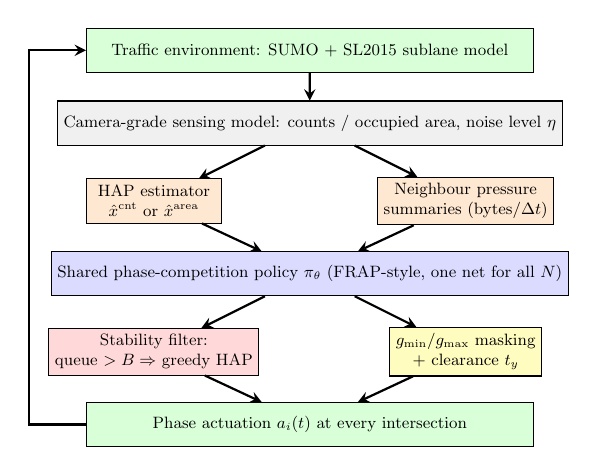
\begin{tikzpicture}[scale=0.66, transform shape,
    block/.style ={rectangle, draw, minimum height=0.85cm,
                   minimum width=2.6cm, align=center, font=\small},
    wide/.style  ={rectangle, draw, minimum height=0.85cm,
                   minimum width=8.6cm, align=center, font=\small},
    arr/.style={->, >=stealth, thick}]
\node[wide, fill=green!15] (env) at (0,5.4)
    {Traffic environment: SUMO $+$ SL2015 sublane model};
\node[wide, fill=gray!12] (sense) at (0,4.0)
    {Camera-grade sensing model: counts / occupied area,
     noise level $\eta$};
\node[block, fill=orange!18] (est) at (-3.0,2.5)
    {HAP estimator\\ $\hat{x}^{\mathrm{cnt}}$ or $\hat{x}^{\mathrm{area}}$};
\node[block, fill=orange!18] (nbr) at (3.0,2.5)
    {Neighbour pressure\\ summaries (bytes/$\Delta t$)};
\node[wide, fill=blue!14] (pol) at (0,1.1)
    {Shared phase-competition policy $\pi_\theta$
     (FRAP-style, one net for all $N$)};
\node[block, fill=red!15] (filt) at (-3.0,-0.4)
    {Stability filter:\\ queue $>B \Rightarrow$ greedy HAP};
\node[block, fill=yellow!25] (mask) at (3.0,-0.4)
    {$g_{\min}$/$g_{\max}$ masking\\ $+$ clearance $t_y$};
\node[wide, fill=green!15] (act) at (0,-1.8)
    {Phase actuation $a_i(t)$ at every intersection};
\draw[arr] (env) -- (sense);
\draw[arr] (sense) -- (est);
\draw[arr] (sense) -- (nbr);
\draw[arr] (est) -- (pol);
\draw[arr] (nbr) -- (pol);
\draw[arr] (pol) -- (filt);
\draw[arr] (pol) -- (mask);
\draw[arr] (filt) -- (act);
\draw[arr] (mask) -- (act);
\draw[arr] (act.west) -- ++(-1.1,0) |- (env.west);
\end{tikzpicture}
\caption{HAPLight architecture. A single shared policy refines the greedy
HAP controller; the stability filter guarantees that congestion behaviour
never falls below the throughput-optimal floor
(Corollary~\ref{cor:filter}).}
\label{fig:arch}
\end{figure}

% ===========================================================================
\section{Experimental Setup}
\label{sec:setup}

\subsection{Pre-Registered Hypotheses and Effect Threshold}
\label{subsec:hypotheses}
To guard against the over-claiming documented in this
field~\cite{b_resco}, we state in advance the hypotheses the experiments
are designed to test, and---equally important---the effect size below
which we will call a difference practically irrelevant regardless of its
$p$-value.

\begin{itemize}
\item \textbf{MPE (minimum practically relevant effect).} We pre-register
      $2\%$ relative improvement in average travel time and $5\%$ in
      weighted average queue length. With $150$ paired samples per
      comparison, Wilcoxon tests detect far smaller differences than
      this; effects below the MPE will be reported as
      \emph{statistically detectable but practically negligible}.
\item \textbf{H1 (heterogeneity-aware pressure matters).} Greedy HAP
      outperforms count-based max-pressure~\cite{b_varaiya} and
      Efficient-MP~\cite{b_efficientmp} under heterogeneous Indian demand
      on weighted and passenger-weighted metrics, by at least the MPE.
\item \textbf{H2 (learning refines the floor).} HAPLight-RL outperforms
      greedy HAP and is at least competitive with
      Advanced-MPLight~\cite{b_advxlight} on all scenarios, with the
      stability filter active in fewer than $5\%$ of decisions under
      nominal demand.
\item \textbf{H3 (robustness).} As $\eta$ grows, area-based HAP and
      noise-randomised HAPLight-RL degrade more slowly than count-based
      baselines; we report the crossover level at which the ordering of
      any two methods reverses.
\item \textbf{H4 (guaranteed floor has no nominal cost).} Enabling the
      filter does not degrade nominal performance by more than the MPE,
      and prevents queue growth under the surge stress test.
\item \textbf{H5 (weight vector matters).} Dynamic-area weights $\pi$
      yield a smaller realised estimator error than Indo-HCM weights
      $\rho^{\mathrm{hcm}}$ (predicted exactly by
      Lemma~\ref{lem:area}), and at least equal control performance.
\end{itemize}
Results that refute any hypothesis will be reported as such.

\subsection{Simulation Environment}
All experiments use SUMO~\cite{b_sumo} through \texttt{libsumo} (rather
than TraCI) for throughput, with the SL2015 sublane model so that
two-wheelers occupy lateral gaps, approximating Indian gap-filling
behaviour~\cite{b_simtram}. Table~\ref{tab:vehicles} gives the complete
vehicle-class specification; these values determine both the simulation
and, through Eq.~\eqref{eq:areadef}, the dynamic-area equivalency vector,
so the two are consistent by construction. Table~\ref{tab:simparams}
gives the remaining simulation parameters. Emissions use SUMO's
HBEFA-based models~\cite{b_hbefa}.

\begin{table*}[htbp]
\caption{Vehicle-class specification. $L,W$ are SUMO \texttt{length} and
\texttt{width}; $g$, $g^{\mathrm{lat}}$ are \texttt{minGap} and
\texttt{minGapLat}. Effective dynamic area $a_v=(L+g)(W+g^{\mathrm{lat}})$
per Eq.~\eqref{eq:areadef}; $\pi_v=a_v/a_c$ is the area equivalency and
$\rho^{\mathrm{hcm}}_v$ the Indo-HCM PCU factor~\cite{b_indohcm};
$\beta_v=a_v/\rho^{\mathrm{hcm}}_v$ drives the bound of
Lemma~\ref{lem:area}. Occupancies are nominal design values applied
identically to all controllers.}
\label{tab:vehicles}
\centering
\footnotesize
\begin{tabular}{@{}lrrrrrrrrrrrr@{}}
\toprule
Class & $L$ (m) & $W$ (m) & $g$ (m) & $g^{\mathrm{lat}}$ (m) &
$v_{\max}$ (km/h) & accel & decel & share &
$a_v$ (m$^2$) & $\pi_v$ & $\rho^{\mathrm{hcm}}_v$ & $\beta_v$ \\
\midrule
Two-wheeler   & 1.90  & 0.70 & 1.00 & 0.20 & 60 & 2.5 & 4.5 & 0.40 & 2.61  & 0.228 & 0.5 & 5.220 \\
Car           & 3.70  & 1.60 & 1.50 & 0.60 & 70 & 2.0 & 4.0 & 0.35 & 11.44 & 1.000 & 1.0 & 11.440 \\
Auto-rickshaw & 2.60  & 1.40 & 1.20 & 0.40 & 45 & 1.5 & 3.5 & 0.10 & 6.84  & 0.598 & 1.2 & 5.700 \\
Bus           & 10.50 & 2.50 & 2.00 & 0.80 & 50 & 1.0 & 3.0 & 0.10 & 41.25 & 3.606 & 3.0 & 13.750 \\
Truck (LCV)   & 7.50  & 2.50 & 2.00 & 0.80 & 50 & 1.0 & 3.0 & 0.05 & 31.35 & 2.740 & 3.5 & 8.957 \\
\midrule
\multicolumn{9}{@{}l}{Nominal passenger occupancy (2W / car / auto / bus / truck)}
 & \multicolumn{4}{r@{}}{$1.3\;/\;1.6\;/\;2.2\;/\;35\;/\;1.5$} \\
\multicolumn{9}{@{}l}{Lemma~\ref{lem:area} under $\rho^{\mathrm{hcm}}$:
 $\bar a^\star=9.485$ m$^2$/PCU, $\varepsilon^\star=0.450$}
 & \multicolumn{4}{r@{}}{under $\pi$: $\bar a=a_c=11.44$, $\varepsilon^\star=0$} \\
\bottomrule
\end{tabular}
\end{table*}

\begin{table}[htbp]
\caption{Simulation and protocol parameters.}
\label{tab:simparams}
\centering
\footnotesize
\begin{tabularx}{\columnwidth}{@{}Xr@{}}
\toprule
Parameter & Value \\
\midrule
Simulation step & 1 s \\
Decision interval $\Delta t$ & 5 s \\
Minimum green $g_{\min}$ & 10 s \\
Maximum green / starvation bound $g_{\max}$ & 120 s \\
Clearance $t_y$ (yellow $+$ all-red) & 3 s $+$ 2 s \\
Lateral resolution (\texttt{lateralResolution}) & 0.8 m \\
Two-wheeler \texttt{latAlignment} / \texttt{lcSublane} & arbitrary / 1.0 \\
Car \texttt{latAlignment} & centre \\
Episode length & 3600 s (720 decisions) \\
Evaluation episodes per seed & 30 \\
Robustness episodes per seed per $\eta$ & 20 \\
Independent seeds & 5 \\
Noise grid $\eta$ (train $\subseteq [0,0.6]$) & $\{0,.2,.4,.6,.8,1.0\}$ \\
Noise maxima $(\theta_{\max},q_{\max},\sigma_{\max})$ & $(0.5,\,0.35,\,0.30)$ \\
\bottomrule
\end{tabularx}
\end{table}

\subsection{Network Scenarios}
\label{subsec:scenarios}
\subsubsection{Scenario 1: 5-intersection arterial}
Five equally spaced signalised intersections at 400~m spacing, for
controlled analysis of coordination and green-wave formation.

\subsubsection{Scenario 2: $4\times4$ grid}
Sixteen intersections in a uniform grid at 300~m spacing, the scale at
which network-level methods are separated in the benchmark
literature~\cite{b_mplight,b_advxlight}.

\subsubsection{Scenario 3: Bengaluru real-world corridor}
A network extracted from OpenStreetMap with SUMO's
\texttt{osmWebWizard}, covering the Old Madras Road (NH-75) arterial and
adjoining town network around Hoskote--K.\,R.~Puram in the Bengaluru
Metropolitan Region, bounding box
$[77.67,\,12.99] \times [77.80,\,13.08]$ (WGS84). The raw export is
processed with \texttt{netconvert} using
\texttt{--junctions.join}, \texttt{--tls.guess-signals} and
\texttt{--tls.join} to repair the unsignalised and fragmented junctions
that OSM exports of Indian arterials typically contain; the resulting
network contains \note{N after extraction and cleanup;
build\_nets.py} signalised intersections. Every manual correction is
recorded in the build script so the network is reproducible from the
bounding box alone. The corridor mixes a high-speed arterial with dense
town junctions and strongly heterogeneous approach geometries, and
carries pronounced directional peaks toward Bengaluru in the morning.

\begin{figure}[htbp]
\centering
\begin{subfigure}[b]{0.14\textwidth}
\centering
\resizebox{\linewidth}{!}{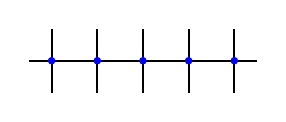
\begin{tikzpicture}[scale=0.29]
    \draw[thick](-1,0)--(9,0);
    \foreach \x in {0,2,4,6,8}{
        \draw[thick](\x,-1.4)--(\x,1.4);
        \filldraw[blue](\x,0)circle(4pt);}
\end{tikzpicture}}
\caption{Scenario 1}
\end{subfigure}
\hfill
\begin{subfigure}[b]{0.15\textwidth}
\centering
\resizebox{\linewidth}{!}{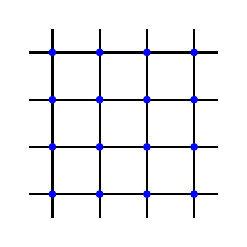
\begin{tikzpicture}[scale=0.30]
    \foreach \x in {0,2,4,6}{\draw[thick](\x,-1)--(\x,7);}
    \foreach \y in {0,2,4,6}{\draw[thick](-1,\y)--(7,\y);}
    \foreach \x in {0,2,4,6}{
        \foreach \y in {0,2,4,6}{\filldraw[blue](\x,\y)circle(4pt);}}
\end{tikzpicture}}
\caption{Scenario 2}
\end{subfigure}
\hfill
\begin{subfigure}[b]{0.14\textwidth}
\centering
\resizebox{\linewidth}{!}{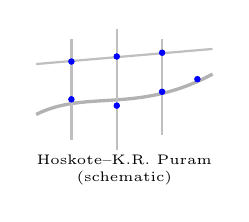
\begin{tikzpicture}[scale=0.32]
    \draw[very thick,gray!60](0,1)..controls(2,2)and(4,1)..(7,2.6);
    \draw[thick,gray!50](1.4,0)--(1.4,4);
    \draw[thick,gray!50](3.2,-0.4)--(3.2,4.4);
    \draw[thick,gray!50](5.0,0.2)--(5.0,4.0);
    \draw[thick,gray!50](0,3)--(7,3.6);
    \foreach \p in {(1.4,1.6),(3.2,1.35),(5.0,1.9),(1.4,3.1),
                    (3.2,3.3),(5.0,3.45),(6.4,2.4)}{
        \filldraw[blue]\p circle(3pt);}
    \node[font=\tiny,align=center]at(3.5,-1.2){Hoskote--K.R.~Puram\\(schematic)};
\end{tikzpicture}}
\caption{Scenario 3}
\end{subfigure}
\caption{Network topologies. \note{Replace panel (c) with the SUMO-GUI
export of the extracted corridor; build\_nets.py}}
\label{fig:topologies}
\end{figure}

\subsection{Traffic Demand}
Vehicle composition follows the shares in Table~\ref{tab:vehicles}
(40\% two-wheelers, 35\% cars, 10\% auto-rickshaws, 10\% buses, 5\%
trucks), representative of Indian urban arterials. Arrival rates follow a
two-peak diurnal profile; Scenario 3 additionally applies a directional
morning peak toward Bengaluru. A \emph{surge stress test} doubles demand
on one approach for 15 minutes mid-episode to probe saturation behaviour
(H4). Because origin--destination data for the corridor is not available
to us, demand is synthetic and composition-calibrated; this is recorded
as a limitation in Sec.~\ref{sec:limitations}, and we additionally report
performance under composition shifts of $\pm10$ percentage points in the
two-wheeler share (Sec.~\ref{subsec:sensitivity}). Passenger-weighted
metrics use the nominal occupancies of Table~\ref{tab:vehicles}, applied
identically to every controller so that comparisons are invariant to
their exact values; sensitivity to bus occupancy in $\{25,40\}$ is
reported.

\subsection{Baselines}
\label{subsec:baselines}
(1)~\textbf{FT}: Webster fixed-time~\cite{b_webster} from Indo-HCM
saturation flows; (2)~\textbf{SOTL}~\cite{b_sotl};
(3)~\textbf{MP}: count-based max-pressure~\cite{b_varaiya};
(4)~\textbf{Efficient-MP}~\cite{b_efficientmp};
(5)~\textbf{Advanced-MP}~\cite{b_advxlight};
(6)~\textbf{Greedy HAP} (ours, Layer 1; both estimators, both weight
vectors); (7)~\textbf{IPPO}: independent PPO without parameter sharing;
(8)~\textbf{PressLight}~\cite{b_presslight};
(9)~\textbf{MPLight}~\cite{b_mplight};
(10)~\textbf{CoLight}~\cite{b_colight};
(11)~\textbf{Advanced-MPLight}~\cite{b_advxlight} (state of the art);
(12)~\textbf{MARDDPG}~\cite{b_marddpg}.

All learning baselines are trained with the same budget, demand
distribution and seeds as HAPLight-RL, and evaluated with the same
protocol; classical baselines receive the same corrupted observations as
learning methods in robustness studies. To keep the protocol within the
compute budget of Sec.~\ref{subsec:compute}, the learned baselines on
Scenario 3 are restricted a priori to
$\{$IPPO, MPLight, Advanced-MPLight, HAPLight-RL$\}$; PressLight,
CoLight and MARDDPG are reported on Scenarios 1 and 2 only. This
restriction is declared here rather than chosen after seeing results.

\subsection{Metrics and Statistics}
\label{subsec:stats}
We report average travel time (ATT), average waiting time (AWT),
weighted average queue length (AQL), average delay (AD), throughput (TP,
veh/h), passenger-weighted delay (PWD), fuel consumption and CO$_2$
(HBEFA), and the Gini coefficient of per-vehicle waiting time overall and
per class.

Each method is run for 30 evaluation episodes on each of 5 seeds, giving
150 paired episode means per comparison. Significance is assessed by
two-sided Wilcoxon signed-rank tests of HAPLight-RL against each baseline
on per-episode means, with Holm--Bonferroni correction applied within
each (scenario, metric) family. Because $n=150$ makes trivially small
differences significant, we additionally report (i)~the rank-biserial
correlation as a non-parametric effect size and (ii)~BCa bootstrap
$95\%$ confidence intervals on the relative difference, and we judge
claims against the pre-registered MPE of
Sec.~\ref{subsec:hypotheses}. A result is described as an improvement
only if it is both corrected-significant and exceeds the MPE.

\subsection{Compute Budget}
\label{subsec:compute}
The protocol is deliberately sized to run on a single workstation, which
we regard as a reproducibility requirement rather than a concession.
Table~\ref{tab:budget} accounts for it. Training uses
$N_{\mathrm{it}}=100$ PPO iterations of $E=8$ parallel episodes, i.e.\
800 episodes per run; with $\Delta t=5$~s and 3600~s episodes this is
$5.76\times10^5$ decision steps per run and $9.2\times10^6$
intersection-transitions on Scenario 2. Because the policy has only
$23{,}650$ parameters, the bottleneck is SUMO rather than gradient
computation, so training runs on CPU with all cores devoted to parallel
environments; no GPU is required. Sublane simulation costs roughly
$2$--$4\times$ the default model, which is accounted for in the budget.

\begin{table}[htbp]
\caption{Compute budget. Episode counts are design values; wall-clock is
measured on the reference machine.}
\label{tab:budget}
\centering
\footnotesize
\begin{tabularx}{\columnwidth}{@{}Xrrr@{}}
\toprule
Stage & S1 & S2 & S3 \\
\midrule
RL methods trained            & 6      & 6      & 4 \\
Seeds                         & 5      & 5      & 5 \\
Episodes per training run     & 800    & 800    & 800 \\
Training episodes (total)     & 24{,}000 & 24{,}000 & 16{,}000 \\
Main-evaluation episodes      & 1{,}800  & 1{,}800  & 1{,}500 \\
Robustness episodes           & ---      & 3{,}600  & 2{,}400 \\
\midrule
Mean wall-clock per episode (s) & \pl & \pl & \pl \\
Total wall-clock (h, 8 cores)   & \pl & \pl & \pl \\
\bottomrule
\end{tabularx}
\end{table}

Table~\ref{tab:hyper} lists the learning hyperparameters.

\begin{table}[htbp]
\caption{HAPLight-RL hyperparameters. $c_{\mathrm{sw}}$ and $B$ are
examined in the sensitivity analysis of Sec.~\ref{subsec:sensitivity}.}
\label{tab:hyper}
\centering
\footnotesize
\begin{tabularx}{\columnwidth}{@{}Xr@{}}
\toprule
Parameter & Value \\
\midrule
Optimiser / learning rate & Adam / $3\times10^{-4}$, linear decay \\
PPO clip / epochs / minibatch & 0.2 / 4 / 512 \\
Discount $\gamma$ / GAE $\lambda$ & 0.99 / 0.95 \\
Entropy coefficient / value coefficient & 0.01 / 0.5 \\
Gradient-norm clip & 0.5 \\
Movement embedding / trunk width & 64 / 64 \\
Total shared parameters & 23{,}650 (92.4 KiB) \\
Switching penalty $c_{\mathrm{sw}}$ & 0.05 \\
Filter threshold $B$ & $P_{90}$ of greedy-HAP queue mass \\
PPO iterations $N_{\mathrm{it}}$ / parallel episodes $E$ & 100 / 8 \\
Training episodes per run & 800 \\
Observation normalisation $x_{\mathrm{ref}},\mu_{\mathrm{ref}}$ & 50, 1.0 \\
\bottomrule
\end{tabularx}
\end{table}

% ===========================================================================
\section{Results and Discussion}
\label{sec:results}
\note{Every value in this section must be produced by the actual
experiments. The tables define the required format. Do not submit until
all placeholders are filled and the narrative is rewritten to match what
the data show, including any refuted hypotheses.}

\subsection{Calibration: Testing the Framework's Own Assumptions}
\label{subsec:calibration}
Two quantities that the theory of Sec.~\ref{sec:theory} treats as given
are in fact empirical. We measure them before any control comparison,
because the rest of the paper is conditional on them.

\subsubsection{C1---Realised estimator error}
We log $(\hat{x}^{\mathrm{area}}_m(t),\,x_m(t))$ for every movement and
decision instant over the nominal demand, and report the distribution of
the ratio. Lemma~\ref{lem:area} predicts support within
$[\beta_{\min}/\bar a,\,\beta_{\max}/\bar a]$, i.e.\ $[0.550,\,1.450]$
under Indo-HCM weights and $\{1\}$ under area weights, with concentration
near $1.052$ for realistic compositions (Remark~\ref{rem:realised}).

\begin{table}[htbp]
\caption{Realised area-estimator error, Scenario 2, nominal demand.
Percentiles of $\hat{x}^{\mathrm{area}}_m/x_m$ over all $(m,t)$.}
\label{tab:calib_eps}
\centering
\footnotesize
\begin{tabularx}{\columnwidth}{@{}Xrrrrr@{}}
\toprule
Weight vector & $P_1$ & $P_{25}$ & median & $P_{75}$ & $P_{99}$ \\
\midrule
Indo-HCM $\rho^{\mathrm{hcm}}$ ($\varepsilon^\star=0.450$) & \pl & \pl & \pl & \pl & \pl \\
Dynamic area $\pi$ ($\varepsilon^\star=0$)                 & \pl & \pl & \pl & \pl & \pl \\
\bottomrule
\end{tabularx}
\end{table}

The measured $99$th-percentile deviation is the value of $\varepsilon$
used when instantiating Proposition~\ref{prop:robust} numerically.

\subsubsection{C2---Composition invariance of saturation flow (A5)}
On a saturated single approach we sweep the two-wheeler share from $0\%$
to $70\%$ (rebalancing the remaining classes proportionally) and measure
the discharge rate during effective green in three unit systems: vehicles
per second, Indo-HCM PCU per second, and area-equivalency units per
second. Assumption~\ref{as:a5} predicts a flat curve in the weighted
units and a strongly increasing curve in vehicles per second.

\begin{table}[htbp]
\caption{Saturation discharge versus composition (Assumption~\ref{as:a5}).
Coefficient of variation of discharge rate across the two-wheeler-share
sweep; smaller is better. A5 is supported if the weighted columns are
flat and counts are not.}
\label{tab:calib_a5}
\centering
\footnotesize
\begin{tabularx}{\columnwidth}{@{}Xrrr@{}}
\toprule
Unit system & min & max & CV (\%) \\
\midrule
Vehicles / s                     & \pl & \pl & \pl \\
Indo-HCM PCU / s                 & \pl & \pl & \pl \\
Area-equivalency units / s       & \pl & \pl & \pl \\
\bottomrule
\end{tabularx}
\end{table}

\note{If the weighted CV is not materially smaller than the count CV,
Assumption~\ref{as:a5} is not supported and Theorem~\ref{thm:stability}
must be restated as conditional; report this outcome honestly and discuss
it in Sec.~\ref{sec:limitations}. Do not proceed as if the assumption
held.}

\subsection{Main Comparison}
\label{subsec:main}

\begin{table*}[htbp]
\caption{Performance comparison. Mean $\pm$ std over 30 evaluation
episodes $\times$ 5 seeds. $\dagger$: $p<0.05$ vs.\ HAPLight-RL after
Holm--Bonferroni correction (Wilcoxon signed-rank);
$\ddagger$: additionally exceeds the pre-registered MPE. Bold $=$ best.}
\label{tab:main}
\centering
\footnotesize
\begin{tabular}{@{}llcccccc@{}}
\toprule
Scenario & Algorithm & ATT (s) & AWT (s) & AQL (units) & TP (veh/h) &
PWD (s) & CO$_2$ (kg) \\
\midrule
\multirow{6}{*}{S1 (arterial)}
 & FT               & \pl & \pl & \pl & \pl & \pl & \pl \\
 & MP               & \pl & \pl & \pl & \pl & \pl & \pl \\
 & Advanced-MP      & \pl & \pl & \pl & \pl & \pl & \pl \\
 & Greedy HAP       & \pl & \pl & \pl & \pl & \pl & \pl \\
 & Advanced-MPLight & \pl & \pl & \pl & \pl & \pl & \pl \\
 & HAPLight-RL      & \pl & \pl & \pl & \pl & \pl & \pl \\
\midrule
\multirow{6}{*}{S2 ($4\times4$)}
 & FT               & \pl & \pl & \pl & \pl & \pl & \pl \\
 & MP               & \pl & \pl & \pl & \pl & \pl & \pl \\
 & Advanced-MP      & \pl & \pl & \pl & \pl & \pl & \pl \\
 & Greedy HAP       & \pl & \pl & \pl & \pl & \pl & \pl \\
 & Advanced-MPLight & \pl & \pl & \pl & \pl & \pl & \pl \\
 & HAPLight-RL      & \pl & \pl & \pl & \pl & \pl & \pl \\
\midrule
\multirow{6}{*}{S3 (Bengaluru)}
 & FT               & \pl & \pl & \pl & \pl & \pl & \pl \\
 & MP               & \pl & \pl & \pl & \pl & \pl & \pl \\
 & Advanced-MP      & \pl & \pl & \pl & \pl & \pl & \pl \\
 & Greedy HAP       & \pl & \pl & \pl & \pl & \pl & \pl \\
 & Advanced-MPLight & \pl & \pl & \pl & \pl & \pl & \pl \\
 & HAPLight-RL      & \pl & \pl & \pl & \pl & \pl & \pl \\
\bottomrule
\end{tabular}
\\[2pt]
\footnotesize
Remaining baselines (SOTL, Efficient-MP, IPPO, PressLight, MPLight,
CoLight, MARDDPG) and the AD metric appear in the extended table of the
supplementary material.
\end{table*}

\begin{table}[htbp]
\caption{Effect sizes for the headline comparisons on Scenario 2:
rank-biserial correlation $r$ and BCa bootstrap 95\% CI on the relative
ATT difference (negative favours HAPLight-RL).}
\label{tab:effect}
\centering
\footnotesize
\begin{tabularx}{\columnwidth}{@{}Xrrr@{}}
\toprule
HAPLight-RL vs. & $r$ & rel.\ $\Delta$ATT (\%) & 95\% CI \\
\midrule
Greedy HAP        & \pl & \pl & \pl \\
Advanced-MP       & \pl & \pl & \pl \\
MPLight           & \pl & \pl & \pl \\
Advanced-MPLight  & \pl & \pl & \pl \\
\bottomrule
\end{tabularx}
\end{table}

\subsection{Effect of the Weight Vector (H5)}
\label{subsec:weightvec}
\note{Report greedy HAP and HAPLight-RL under $\rho^{\mathrm{hcm}}$ vs.\
$\pi$, each with the count and area estimators (four cells), on
Scenario 2 at $\eta=0$ and $\eta=0.6$. Lemma~1 predicts the area/$\pi$
cell is exact and the area/HCM cell carries the largest bias; state
whether control performance follows the prediction.}

\subsection{Robustness to Sensing Noise (H3)}
\label{subsec:robustness}
\begin{figure}[htbp]
\centering
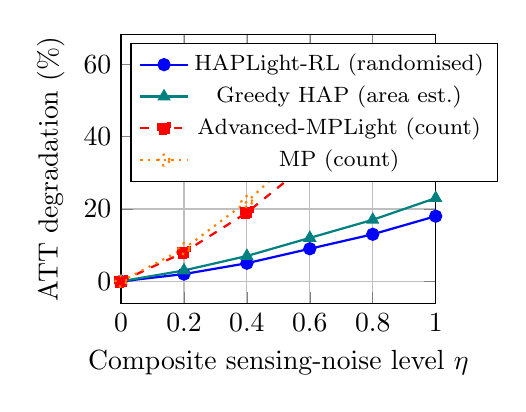
\begin{tikzpicture}
\begin{axis}[
    width=0.46\textwidth, height=5cm,
    xlabel={Composite sensing-noise level $\eta$},
    ylabel={ATT degradation (\%)},
    legend pos=north west, legend style={font=\footnotesize},
    grid=major, xmin=0, xmax=1]
% FORMAT ONLY. Replace every coordinate with measured values.
% Shade eta>0.6 to mark the out-of-training-distribution region.
\addplot[blue, thick, mark=*] coordinates {
    (0,0)(0.2,2)(0.4,5)(0.6,9)(0.8,13)(1.0,18)};
\addlegendentry{HAPLight-RL (randomised)}
\addplot[teal, thick, mark=triangle*] coordinates {
    (0,0)(0.2,3)(0.4,7)(0.6,12)(0.8,17)(1.0,23)};
\addlegendentry{Greedy HAP (area est.)}
\addplot[red, thick, dashed, mark=square*] coordinates {
    (0,0)(0.2,8)(0.4,19)(0.6,33)(0.8,44)(1.0,55)};
\addlegendentry{Advanced-MPLight (count)}
\addplot[orange, thick, dotted, mark=o] coordinates {
    (0,0)(0.2,9)(0.4,22)(0.6,38)(0.8,50)(1.0,62)};
\addlegendentry{MP (count)}
\end{axis}
\end{tikzpicture}
\caption{Degradation of travel time as the composite sensing-noise level
$\eta$ increases (Scenario 2). Levels $\eta>0.6$ lie outside the
training range. \note{Replace all curves with measured values and shade
the out-of-distribution region; evaluate.py}}
\label{fig:robustness}
\end{figure}

\subsection{Ablation Study}
\label{subsec:ablation}
\begin{table*}[htbp]
\caption{Ablations on Scenario 2. Each row removes or replaces one
component of full HAPLight-RL. Rows A and A$'$ jointly isolate the two
distinct claims made about the reward in Sec.~\ref{subsec:reward}.}
\label{tab:ablation}
\centering
\footnotesize
\begin{tabular}{@{}clcccc@{}}
\toprule
Variant & Description & ATT (s) & AWT (s) & AQL (units) & Filter act.\ (\%) \\
\midrule
A  & Count-based ($\rho\equiv1$) queue reward in place of the HAP reward & \pl & \pl & \pl & \pl \\
A$'$ & Unweighted pressure reward $-\sum_m w_m$ (drops $\mu_m$; PressLight-style) & \pl & \pl & \pl & \pl \\
B  & Per-intersection networks in place of the shared policy & \pl & \pl & \pl & \pl \\
C  & Neighbour pressure summaries removed from the observation & \pl & \pl & \pl & \pl \\
D  & Domain randomisation disabled (trained clean; evaluated clean and noisy) & \pl & \pl & \pl & \pl \\
E  & Stability filter disabled (nominal and surge stress test) & \pl & \pl & \pl & --- \\
E$'$ & Filter enabled but overridden steps included in the policy loss & \pl & \pl & \pl & \pl \\
F  & Switching penalty $c_{\mathrm{sw}}=0$ & \pl & \pl & \pl & \pl \\
G  & HAPLight-RL (full) & \pl & \pl & \pl & \pl \\
\bottomrule
\end{tabular}
\end{table*}

\subsection{Fairness and Per-Class Outcomes}
\begin{table}[htbp]
\caption{Per-class average waiting time (s) and Gini coefficient of
per-vehicle waiting time, Scenario 3.}
\label{tab:fairness}
\centering
\footnotesize
\begin{tabularx}{\columnwidth}{@{}Xrrrrrr@{}}
\toprule
Algorithm & 2W & Car & Auto & Bus & Truck & Gini \\
\midrule
FT               & \pl & \pl & \pl & \pl & \pl & \pl \\
MP               & \pl & \pl & \pl & \pl & \pl & \pl \\
Greedy HAP       & \pl & \pl & \pl & \pl & \pl & \pl \\
Advanced-MPLight & \pl & \pl & \pl & \pl & \pl & \pl \\
HAPLight-RL      & \pl & \pl & \pl & \pl & \pl & \pl \\
\bottomrule
\end{tabularx}
\end{table}

\note{Space-equivalency weighting deliberately de-prioritises
two-wheelers relative to counts (a 2W is charged 0.228--0.5 of a car).
Check explicitly whether 2W waiting time worsens under HAP relative to
count-based MP. If it does, say so plainly: it is the predictable price
of the weighting, and the passenger-weighted and Gini columns are where
the trade-off must be justified.}

\subsection{Surge Stress Test and Filter Behaviour (H4)}
\label{subsec:surge}
\note{Report: time series of total weighted queue during the surge for
HAPLight-RL with and without the filter; the filter activation timeline;
recovery time to pre-surge queue levels; and the $g_{\max}$ override
activation frequency (Proposition~\ref{prop:gmax}); compared against
greedy HAP and Advanced-MPLight.}

\begin{remark}[Expect the filter to dominate under saturation]
\label{rem:filterdominates}
Under heavy congestion most intersections exceed $B$, so HAPLight-RL
converges behaviourally to greedy HAP. This is the guarantee working as
designed, not a defect, but it means gains under saturation should
\emph{not} be attributed to learning. The reported activation rate makes
this attribution checkable, and the surge experiment should be read as a
test of the floor rather than of the policy.
\end{remark}

\subsection{Sensitivity Analyses}
\label{subsec:sensitivity}
\note{Report: (i) performance vs.\
$c_{\mathrm{sw}}\in\{0,0.02,0.05,0.1,0.2\}$; (ii) performance and filter
activation vs.\ $B\in\{P_{75},P_{90},P_{97}\}$, alongside the predicted
queue bound of Eq.~(20); (iii) all metrics under equivalency factors
perturbed by $\pm20\%$; (iv) $\Delta t\in\{5,10\}$~s; (v) two-wheeler
share shifted by $\pm10$ percentage points; (vi) bus occupancy
$\in\{25,40\}$ for PWD only.}

\subsection{Training Behaviour}
\begin{figure}[htbp]
\centering
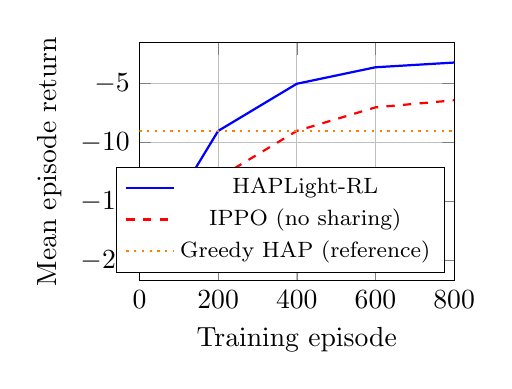
\begin{tikzpicture}
\begin{axis}[
    width=0.46\textwidth, height=4.6cm,
    xlabel={Training episode}, ylabel={Mean episode return},
    legend pos=south east, legend style={font=\footnotesize},
    grid=major, xmin=0, xmax=800]
% FORMAT ONLY. Replace with measured curves (5-seed mean +- 1 std band).
\addplot[blue, thick] coordinates {(0,-20)(200,-9)(400,-5)(600,-3.6)(800,-3.2)};
\addlegendentry{HAPLight-RL}
\addplot[red, thick, dashed] coordinates {(0,-20)(200,-13)(400,-9)(600,-7)(800,-6.4)};
\addlegendentry{IPPO (no sharing)}
\addplot[orange, thick, dotted] coordinates {(0,-9)(800,-9)};
\addlegendentry{Greedy HAP (reference)}
\end{axis}
\end{tikzpicture}
\caption{Training curves on Scenario 2 (format only;
\note{replace with measured curves, 5-seed mean $\pm$ std; train.py}).
The greedy HAP return level is the certified reference the learner must
exceed to justify its existence.}
\label{fig:training}
\end{figure}

% ===========================================================================
\section{Complexity and Deployability}
\label{sec:complexity}

\subsection{Computation}
Greedy HAP costs $O(|\Phi_i|)$ arithmetic per intersection per decision.
HAPLight-RL performs one forward pass of a single shared network of
$23{,}650$ parameters ($92.4$~KiB in fp32) per intersection per
$\Delta t$; total inference cost is linear in $N$ with no centralised
component. At $\Delta t=5$~s the per-intersection compute budget is five
seconds of wall time for a sub-millisecond forward pass, so the
controller is not compute-bound on any plausible hardware;
\note{measured latency on a Raspberry Pi 4 / Jetson Nano class device}.
Training time is reported in Table~\ref{tab:budget}.

\subsection{Sensing and Communication}
The framework needs, per intersection: one camera per approach (or a
single pan installation) providing either classified counts or occupied
area in fixed catchment polygons; and a few bytes per $\Delta t$ of
neighbour pressure exchange over any commodity link. No loop detectors,
no vehicle connectivity, and no central computer are required. The area
estimator's independence from per-class detection
(Sec.~\ref{subsec:estimators}) removes the most failure-prone perception
stage, Lemma~\ref{lem:area} shows this costs nothing when the equivalency
vector is chosen consistently, and Proposition~\ref{prop:robust} bounds
the cost of the residual error---together, a deployment story that
neither SCOOT/SCATS-class systems nor count-based DRL controllers can
offer for Indian conditions.

\subsection{Reproducibility}
All code, network files (including the \texttt{netconvert} invocation and
every manual correction for Scenario 3), demand definitions, trained
models and analysis scripts will be released at
\note{repository URL} upon acceptance, with configuration files
reproducing every table and figure. The compute budget of
Table~\ref{tab:budget} is stated so that the full protocol can be
re-run, not merely inspected.

% ===========================================================================
\section{Limitations}
\label{sec:limitations}
\begin{enumerate}
\item \textbf{Simulation fidelity.} The SL2015 sublane model approximates
      but does not reproduce non-lane-based Indian flow~\cite{b_simtram};
      saturation discharge of mixed queues, in which two-wheelers
      percolate to the front, is only partially captured. The theory is
      simulator-independent, but reported magnitudes are conditional on
      SUMO.
\item \textbf{Assumption A5 is empirical and simulator-conditional.}
      Theorem~\ref{thm:stability} rests on composition-invariant
      saturation flow. We test it (Sec.~\ref{subsec:calibration}) rather
      than assume it, but the test is in simulation; field validation on
      an Indian approach is required before the guarantee can be claimed
      for a deployment.
\item \textbf{Equivalency--estimator coupling.} Lemma~\ref{lem:area}
      shows the classification-free estimator is exact only when the
      equivalency vector is derived from the same area model. Using
      Indo-HCM weights with an area camera incurs a worst-case
      $\varepsilon^\star=0.450$. Practitioners obliged to report in
      Indo-HCM PCU therefore face a real trade-off, which our two-weight
      comparison quantifies but does not remove.
\item \textbf{The area model itself is idealised.} Eq.~\eqref{eq:areadef}
      uses standstill clearances; real dynamic area varies with speed,
      and a field study correlating camera-measured occupied area with
      classified counts remains the necessary next step.
\item \textbf{Synthetic demand.} Scenario 3 uses a real network but
      synthetic, composition-calibrated demand; origin--destination
      calibration from Bengaluru sensor or survey data awaits data
      access.
\item \textbf{Stability is not delay-optimality.} Theorem~\ref{thm:stability}
      certifies bounded queues, not minimal delay; the learned layer
      targets delay empirically, without a guarantee beyond the floor of
      Corollary~\ref{cor:filter}. Moreover the floor is least
      informative where it binds most (Remark~\ref{rem:filterdominates}).
\item \textbf{Pedestrians and non-motorised traffic.} Pedestrian phases
      and non-motorised vehicles are not modelled and materially
      influence Indian junction operation.
\end{enumerate}

% ===========================================================================
\section{Conclusion and Future Work}
\label{sec:conclusion}
This paper reframed heterogeneous-traffic signal control around a
measure---HAP---defined over a general space-equivalency weight vector,
chosen so that a decentralised greedy controller carries a
throughput-optimality proof with its assumptions stated and tested, a
classification-free camera estimator with a \emph{tight} error bound, and
a robustness guarantee under sensing error that correctly charges only
the dispersion of that error. On that foundation we added exactly as much
learning as it justifies: a single shared $23{,}650$-parameter
phase-competition policy, trained with PPO under sensing-noise domain
randomisation with a reward equal to the Lyapunov drift functional, and
wrapped in a filter that provably preserves the classical guarantee with
an explicit queue bound. The analysis also produced a design rule that
was not visible before the bound was made tight: the equivalency vector
and the camera estimator must be derived from the same area model, or the
classification-free pipeline pays a worst-case $45\%$ error for nothing.

Future work includes: field validation of the area estimator and the
composition-invariance assumption, and a pilot deployment with fail-safe
supervision; pedestrian and non-motorised integration into the HAP
formulation; origin--destination calibration from Bengaluru data;
extension of the robustness theory to time-varying demand and
\emph{systematic} estimation bias, which Remark~\ref{rem:dispersion}
shows behaves quite differently from dispersed error; and multi-objective
extensions (emissions, per-class equity) within the certified-floor
architecture.

% ===========================================================================
\section*{Acknowledgment}
The authors thank the Department of Computer Science and Engineering and
the Department of Mathematics and Computing, Rajiv Gandhi Institute of
Petroleum Technology, for computational resources.

% ===========================================================================
\appendices

\section{Proof of Theorem~\ref{thm:stability}}
\label{app:thm1}
Work in slots of length $\Delta t$ and let $X(t)=(x_m(t))_m$ be the
vector of weighted queues. The dynamics are
\begin{equation}
x_m(t+1) = \big[x_m(t) - y_m(t)\big]^+ + a_m(t)
           + \sum_{m'} r_{m'm}\, y_{m'}(t),
\label{eq:dynamics}
\end{equation}
where $y_m(t) \le \min\{x_m(t),\, \mu_m \Delta t\, S_m(t)\}$ is the
weighted mass discharged, $S_m(t)\in\{0,1\}$ the green indicator, and
$a_m(t)$ the exogenous weighted arrival. Assumption~\ref{as:a5} is what
makes $\mu_m$ a constant here rather than a function of the queue's class
composition.

Take $V(X)=\tfrac12\sum_m x_m^2$. Using
$([x-y]^+ + z)^2 \le x^2 + y^2 + z^2 - 2x(y-z)$ and taking conditional
expectations,
\begin{equation}
\begin{aligned}
\mathbb{E}[V(t{+}1)&-V(t)\mid X]\\
 &\le K - \sum_m x_m\, \mathbb{E}\Big[y_m - a_m
   - \textstyle\sum_{m'} r_{m'm} y_{m'} \,\Big|\, X\Big],
\end{aligned}
\label{eq:drift0}
\end{equation}
where $K$ absorbs all second-order terms. $K$ is finite because per-slot
weighted arrivals and departures are bounded
(Assumptions~\ref{as:a1},~\ref{as:a4}); this is the only point at which
vehicle-type randomness enters, through bounded second moments of the
weighted masses, and it does so harmlessly.

Exchanging the order of summation in the routing term,
\begin{equation}
\sum_m x_m \sum_{m'} r_{m'm} y_{m'}
 = \sum_{m} y_{m} \sum_{m'} r_{mm'} x_{m'},
\end{equation}
so the service terms of~\eqref{eq:drift0} collapse to
\begin{equation}
\sum_m y_m \Big( x_m - \sum_{m'} r_{mm'} x_{m'} \Big)
 = \sum_m y_m\, w_m(t),
\label{eq:collapse}
\end{equation}
with $w_m$ exactly as defined in Eq.~\eqref{eq:weight}. Substituting
$y_m = \mu_m \Delta t\, S_m$ (the correction in the saturated case
$x_m < \mu_m\Delta t$ is standard and bounded),
\begin{equation}
\sum_m y_m w_m = \Delta t \sum_{i\in\mathcal{I}}
 \sum_{m\in\phi_i} \mu_m w_m = \Delta t \sum_i P_i(\phi_i,t),
\end{equation}
which is separable across intersections. Hence the greedy
choice~\eqref{eq:greedy} maximises the whole functional globally, and
\begin{equation}
\mathbb{E}[\Delta V \mid X] \le K + \Delta t\sum_m x_m \lambda_m
 - \Delta t \sum_i \max_{\phi} P_i(\phi,t).
\label{eq:drift1}
\end{equation}

By Assumption~\ref{as:a3} there exist $\delta>0$ and a stationary
randomised phase-selection rule whose expected net service exceeds
arrivals by margin $\delta$ componentwise. The greedy policy's max-weight
value dominates that of any randomised rule pointwise in $X$, so
\begin{equation}
\mathbb{E}[\Delta V \mid X] \;\le\; K - \delta \sum_m x_m
\end{equation}
whenever $\sum_m x_m$ is large. The Foster--Lyapunov drift criterion then
yields strong stability with
$\limsup_T \frac1T\sum_t \mathbb{E}[\sum_m x_m(t)] \le K/\delta$, which
is Eq.~\eqref{eq:stability}.

Two observations complete the argument. First, no step used
$\rho\equiv1$: the derivation holds verbatim for any strictly positive
weight vector, with $\Lambda$, $\lambda$ and $\mu$ all expressed in the
corresponding units. Second, the derivation \emph{did} use
Assumption~\ref{as:a5} at Eq.~\eqref{eq:dynamics}; a weight vector for
which $\mu_m$ varies with composition invalidates the constant-rate
substitution and with it the theorem. This is the precise sense in which
the choice of units is not cosmetic (Remark~\ref{rem:notunits}).
\hfill$\blacksquare$

\section{Proof of Proposition~\ref{prop:robust}}
\label{app:prop1}
Let $\hat w_m$ be the weights computed from $\hat x$, where
$\hat x_m = (1+\varepsilon_m) x_m$ with $|\varepsilon_m| \le \varepsilon$
varying arbitrarily over $m$ and $t$. Then
\begin{equation}
\begin{aligned}
|\hat w_m - w_m| &\;\le\; |\hat x_m - x_m|
 + \sum_{m'} r_{mm'} |\hat x_{m'} - x_{m'}|\\
 &\;\le\; \varepsilon\Big( x_m + \sum_{m'} r_{mm'} x_{m'}\Big).
\end{aligned}
\end{equation}
For the max-weight functional
$T(w,S) = \Delta t \sum_m \mu_m w_m S_m$ over feasible phase profiles
$S$,
\begin{align}
|T(\hat w,S) - T(w,S)|
&\le \Delta t\, \mu_{\max}\, \varepsilon
   \sum_m \Big( x_m + \sum_{m'} r_{mm'} x_{m'} \Big) \nonumber\\
&\le \Delta t\, \mu_{\max}\, \varepsilon\, (1+K_r)\, \|X\|_1 \nonumber\\
&= \tfrac12 c_1 \Delta t\, \varepsilon \|X\|_1,
\end{align}
using $\sum_m \sum_{m'} r_{mm'} x_{m'} = \sum_{m'} x_{m'}\sum_m r_{mm'}
\le K_r \|X\|_1$ and $c_1 = 2\mu_{\max}(1+K_r)$ as in~\eqref{eq:c1}.

Let $\hat S$ maximise $T(\hat w,\cdot)$ and $S^\star$ maximise
$T(w,\cdot)$. Chaining the three inequalities,
\begin{align}
T(w,\hat S) &\ge T(\hat w,\hat S)
             - \tfrac12 c_1\Delta t\,\varepsilon\|X\|_1 \nonumber\\
            &\ge T(\hat w, S^\star)
             - \tfrac12 c_1\Delta t\,\varepsilon\|X\|_1 \nonumber\\
            &\ge T(w, S^\star) - c_1\Delta t\,\varepsilon\|X\|_1 .
\label{eq:perturb}
\end{align}
Substituting~\eqref{eq:perturb} into the drift bound~\eqref{eq:drift1} of
Appendix~\ref{app:thm1} replaces the margin $\delta$ by
$\delta - c_1\Delta t\,\varepsilon$:
\begin{equation}
\mathbb{E}[\Delta V\mid X] \;\le\; K
 - \big(\delta - c_1 \Delta t\, \varepsilon\big)\, \|X\|_1 ,
\end{equation}
which is negative outside a bounded set precisely when
$\varepsilon < \delta/(c_1\Delta t)$, giving strong stability by
Foster--Lyapunov. Since the interiority margin $\delta(\lambda)$ is
continuous, strictly positive on $\operatorname{int}\Lambda$, and
decreases to $0$ as $\lambda \to \partial\Lambda$ along rays, the set
$\{\lambda : \delta(\lambda) > c_1\Delta t\,\varepsilon\}$ contains a
scaled copy of $\Lambda$; this is the claimed $(1+c\varepsilon)$
interiority condition, with $c$ determined by $\mu_{\max}$, $K_r$,
$\Delta t$ and the geometry of $\Lambda$.

Finally, note where the bound is loose and why this matters. If
$\varepsilon_m(t)\equiv\varepsilon$ is common to all movements, then
$\hat w = (1+\varepsilon) w$ exactly, $\hat S = S^\star$, and the
inequality~\eqref{eq:perturb} holds with zero slack: no capacity is lost
for any $\varepsilon$. The proposition therefore charges only the
\emph{dispersion} of the estimation error across movements, as stated in
Remark~\ref{rem:dispersion}. \hfill$\blacksquare$

\section{Proof of Proposition~\ref{prop:gmax}}
\label{app:prop2}
Partition slots into those in which the $g_{\max}$ override is active at
some intersection and those in which it is not. On non-overridden slots
the drift bound of Appendix~\ref{app:thm1} applies unchanged. On an
overridden slot the executed profile $S^{\mathrm{ov}}$ may differ
arbitrarily from $S^\star$, but both are feasible, so
\begin{equation}
T(w,S^\star) - T(w,S^{\mathrm{ov}}) \;\le\;
 \Delta t\,\mu_{\max}\sum_m |w_m| \;\le\;
 \tfrac12 c_1 \Delta t\, \|X\|_1 ,
\end{equation}
using $\sum_m|w_m| \le (1+K_r)\|X\|_1$ and $c_1$ from~\eqref{eq:c1}.
Applying the $T$-slot drift criterion over a window containing a fraction
$f$ of overridden slots and averaging,
\begin{equation}
\mathbb{E}[\Delta V\mid X] \;\le\; K
 - \big(\delta - \tfrac12 c_1 \Delta t\, f\big)\|X\|_1 ,
\end{equation}
so stability holds whenever $\delta > \tfrac12 c_1\Delta t\, f$.

For the bound on $f$: the override at intersection $i$ fires for phase
$\phi$ only after $\phi$ has been unserved for $g_{\max}$ seconds, and
grants a single service of duration $g_{\min}$, after which $\phi$'s
starvation timer resets. Hence within any window each of the $|\Phi_i|$
phases can trigger at most once, contributing at most
$|\Phi_i| g_{\min}$ overridden seconds per $g_{\max} + |\Phi_i| g_{\min}$
seconds of operation, which is Eq.~\eqref{eq:fbound}. The bound is
worst-case: it assumes every phase starves in every window, whereas
pressure-driven service already prevents most starvation, so the measured
$f$ is typically far smaller. \hfill$\blacksquare$

\section{Proof of Corollary~\ref{cor:filter}}
\label{app:cor1}
Call a queue \emph{large} if it exceeds $B$, and an intersection
\emph{triggered} if any queue entering its pressure computation is large.
Triggered intersections act greedily by construction. The max-weight
functional is separable across intersections
(Appendix~\ref{app:thm1}), so triggered intersections contribute their
maximal local term.

For a non-triggered intersection $i$, all pressure inputs are below $B$,
hence $|w_m| \le B(1+K_r)$ for every $m\in\Mset_i$ and
\begin{equation}
\big|P_i(\phi,t)\big| \;\le\; |\Mset_i|\,\mu_{\max} B (1+K_r)
 \;\le\; c_2 B
\end{equation}
with $c_2 = |\Mset|_{\max}\mu_{\max}(1+K_r)$. The local suboptimality of
an arbitrary action relative to the greedy one is therefore at most
$2c_2 B$, and across $N$ intersections at most $2Nc_2B$---a constant
independent of $X$. The drift bound of Appendix~\ref{app:thm1} becomes
\begin{equation}
\mathbb{E}[\Delta V \mid X] \;\le\; K + 2Nc_2B\Delta t
 - \delta \sum_m x_m ,
\end{equation}
which is negative outside the bounded set
$\{\sum_m x_m > (K + 2Nc_2B\Delta t)/\delta\}$. Foster--Lyapunov yields
strong stability with the bound~\eqref{eq:filterbound}. The
noisy-measurement version follows by combining with
Appendix~\ref{app:prop1}, replacing $\delta$ by
$\delta - c_1\Delta t\,\varepsilon$.

The bound grows linearly in $NB$, which quantifies the design trade-off:
a permissive filter (large $B$) grants the learned policy more autonomy
but weakens the certificate proportionally. \hfill$\blacksquare$

\section{Proof of Lemma~\ref{lem:area}}
\label{app:lemma}
Fix $m$ and $t$ and write $n_v = n_{m,v}(t)$. By
Eqs.~\eqref{eq:xdef} and~\eqref{eq:area_est},
\begin{equation}
\frac{\hat{x}^{\mathrm{area}}_m}{x_m}
 = \frac{\sum_v a_v n_v}{\bar a \sum_v \rho_v n_v}
 = \sum_v \left(\frac{\beta_v}{\bar a}\right)
   \underbrace{\frac{\rho_v n_v}{\sum_{v'} \rho_{v'} n_{v'}}}_{=:\,\omega_v},
\end{equation}
where $\beta_v = a_v/\rho_v$ and we used $a_v = \beta_v \rho_v$. The
weights $\omega_v$ are non-negative and sum to one, so the ratio is a
convex combination of $\{\beta_v/\bar a\}_{v\in\vc}$ and therefore lies
in $[\beta_{\min}/\bar a,\ \beta_{\max}/\bar a]$, which
is~\eqref{eq:lem_bound}. Both endpoints are attained by queues consisting
entirely of the argmin and argmax class respectively, so the bound is
tight without further assumptions on the composition.

For the optimal calibration constant, $\varepsilon(\bar a) =
\max\{\beta_{\max}/\bar a - 1,\ 1 - \beta_{\min}/\bar a\}$ is the maximum
of a strictly decreasing and a strictly increasing function of $\bar a$,
so it is minimised where they are equal, i.e.\ at
$\bar a^\star = \tfrac12(\beta_{\min}+\beta_{\max})$, whence
\begin{equation}
\varepsilon^\star = \frac{\beta_{\max}}{\bar a^\star} - 1
 = \frac{\beta_{\max}-\beta_{\min}}{\beta_{\max}+\beta_{\min}},
\end{equation}
which is Eq.~\eqref{eq:epsstar}. This quantity is scale-free: it is
invariant under $\beta \mapsto \gamma\beta$ for any $\gamma>0$, so it
measures only the \emph{dispersion} of footprint-to-weight ratios and not
their common scale. Finally $\varepsilon^\star=0$ iff
$\beta_{\max}=\beta_{\min}$, i.e.\ iff $a_v/\rho_v$ is constant across
classes, i.e.\ iff $\rho_v \propto a_v$. Substituting the values of
Table~\ref{tab:vehicles} gives $\varepsilon^\star = 0.450$ for
$\rho^{\mathrm{hcm}}$ and $\varepsilon^\star = 0$ for $\pi$.
\hfill$\blacksquare$
\begin{thebibliography}{00}

\bibitem{b_tomtom}
TomTom, ``TomTom Traffic Index,'' 2024. [Online]. Available:
\url{https://www.tomtom.com/traffic-index/}

\bibitem{b_morth}
Ministry of Road Transport and Highways, ``Road Transport Year Book,''
Government of India, New Delhi, 2021.

\bibitem{b_scoot}
P.~B. Hunt, D.~I. Robertson, R.~D. Bretherton, and M.~C. Royle,
``The SCOOT on-line traffic signal optimisation technique,''
\textit{Traffic Eng.\ Control}, vol.~23, no.~4, pp.~190--192, 1982.

\bibitem{b_scats}
P.~Lowrie, ``SCATS: Sydney co-ordinated adaptive traffic system,''
in \textit{Proc.\ Int.\ Conf.\ Road Traffic Signalling}, 1982, pp.~67--70.

\bibitem{b_webster}
F.~V. Webster, ``Traffic signal settings,'' Road Research Technical
Paper No.~39, UK DSIR, 1958.

\bibitem{b_sotl}
S.-B. Cools, C.~Gershenson, and B.~D'Hooghe, ``Self-organizing traffic
lights: A realistic simulation,'' in \textit{Advances in Applied
Self-Organizing Systems}. Springer, 2013, pp.~45--55.

\bibitem{b_varaiya}
P.~Varaiya, ``Max pressure control of a network of signalized
intersections,'' \textit{Transp.\ Res.\ Part C: Emerg.\ Technol.},
vol.~36, pp.~177--195, 2013.

\bibitem{b_tassiulas}
L.~Tassiulas and A.~Ephremides, ``Stability properties of constrained
queueing systems and scheduling policies for maximum throughput in
multihop radio networks,'' \textit{IEEE Trans.\ Autom.\ Control},
vol.~37, no.~12, pp.~1936--1948, 1992.

\bibitem{b_lioris}
J.~Lioris, A.~Kurzhanskiy, and P.~Varaiya, ``Adaptive max pressure
control of network of signalized intersections,''
\textit{IFAC-PapersOnLine}, vol.~49, no.~22, pp.~19--24, 2016.

\bibitem{b_anderson}
L.~Anderson, T.~Pumir, D.~Triantafyllos, and A.~M. Bayen, ``Stability and
implementation of a cycle-based max pressure controller for signalized
traffic networks,'' \textit{Netw.\ Heterog.\ Media}, vol.~13, no.~2,
p.~241, 2018.

\bibitem{b_levin}
M.~W. Levin, J.~Hu, and M.~Odell, ``Max-pressure signal control with
cyclical phase structure,'' \textit{Transp.\ Res.\ Part C: Emerg.\
Technol.}, vol.~120, 2020.

\bibitem{b_efficientmp}
Q.~Wu, L.~Zhang, J.~Shen, L.~L\"u, B.~Du, and J.~Wu, ``Efficient
pressure: Improving efficiency for signalized intersections,''
\textit{arXiv preprint arXiv:2112.02336}, 2021.

\bibitem{b_capacityaware}
A.~A. Zaidi, B.~Kulcs\'ar, and H.~Wymeersch, ``Back-pressure traffic
signal control with fixed and adaptive routing for urban vehicular
networks,'' \textit{IEEE Trans.\ Intell.\ Transp.\ Syst.}, vol.~17,
no.~8, pp.~2134--2143, 2016.

\bibitem{b_cmp}
T.~Ahmed, H.~Liu, and V.~V. Gayah, ``C-MP: A decentralized
adaptive-coordinated traffic signal control using the max pressure
framework,'' \textit{Transp.\ Res.\ Part B: Methodol.}, vol.~200,
p.~103308, 2025.

\bibitem{b_occmp}
T.~Ahmed, H.~Liu, and V.~V. Gayah, ``OCC-MP: A max-pressure framework to
prioritize transit and high occupancy vehicles,'' \textit{Transp.\ Res.\
Part C: Emerg.\ Technol.}, 2024.

\bibitem{b_cvmp}
C.~Tan, D.~Sun, H.~Liu, M.~Rinaldi, and H.~van Lint, ``CV-MP:
Max-pressure control in heterogeneously distributed and partially
connected vehicle environments,'' \textit{Transp.\ Res.\ Part B:
Methodol.}, 2025.

\bibitem{b_thorpe}
T.~L. Thorpe and C.~Anderson, ``Traffic light control using SARSA with
three state representations,'' IBM Tech.\ Rep., 1997.

\bibitem{b_abdulhai}
B.~Abdulhai, R.~Pringle, and G.~J. Karakoulas, ``Reinforcement learning
for true adaptive traffic signal control,'' \textit{J.\ Transp.\ Eng.},
vol.~129, no.~3, pp.~278--285, 2003.

\bibitem{b_intellilight}
H.~Wei, G.~Zheng, H.~Yao, and Z.~Li, ``IntelliLight: A reinforcement
learning approach for intelligent traffic light control,'' in
\textit{Proc.\ ACM SIGKDD}, 2018, pp.~2496--2505.

\bibitem{b_frap}
G.~Zheng \textit{et al.}, ``Learning phase competition for traffic signal
control,'' in \textit{Proc.\ ACM CIKM}, 2019, pp.~1963--1972.

\bibitem{b_presslight}
H.~Wei \textit{et al.}, ``PressLight: Learning max pressure control to
coordinate traffic signals in arterial network,'' in \textit{Proc.\ ACM
SIGKDD}, 2019, pp.~1290--1298.

\bibitem{b_colight}
H.~Wei \textit{et al.}, ``CoLight: Learning network-level cooperation for
traffic signal control,'' in \textit{Proc.\ ACM CIKM}, 2019,
pp.~1913--1922.

\bibitem{b_mplight}
C.~Chen \textit{et al.}, ``Toward a thousand lights: Decentralized deep
reinforcement learning for large-scale traffic signal control,'' in
\textit{Proc.\ AAAI}, 2020, pp.~3414--3421.

\bibitem{b_advxlight}
L.~Zhang, Q.~Wu, J.~Shen, L.~L\"u, B.~Du, and J.~Wu, ``Expression might
be enough: Representing pressure and demand for reinforcement learning
based traffic signal control,'' in \textit{Proc.\ ICML} (PMLR vol.~162),
2022, pp.~26645--26654.

\bibitem{b_ma2c}
T.~Chu, J.~Wang, L.~Codec\`a, and Z.~Li, ``Multi-agent deep
reinforcement learning for large-scale traffic signal control,''
\textit{IEEE Trans.\ Intell.\ Transp.\ Syst.}, vol.~21, no.~3,
pp.~1086--1095, 2020.

\bibitem{b_marddpg}
T.~Wu \textit{et al.}, ``Multi-agent deep reinforcement learning for
urban traffic light control in vehicular networks,'' \textit{IEEE
Trans.\ Veh.\ Technol.}, vol.~69, no.~8, pp.~8243--8256, 2020.

\bibitem{b_heterolight}
Y.~Zhang, P.~Li, M.~Fan, and G.~Sartoretti, ``HeteroLight: A general and
efficient learning approach for heterogeneous traffic signal control,''
in \textit{Proc.\ IEEE/RSJ IROS}, 2024, pp.~1010--1017.

\bibitem{b_resco}
J.~Ault and G.~Sharon, ``Reinforcement learning benchmarks for traffic
signal control,'' in \textit{Proc.\ NeurIPS Datasets and Benchmarks
Track}, 2021.

\bibitem{b_safelight}
W.~Du, J.~Ye, J.~Gu, J.~Li, H.~Wei, and G.~Wang, ``SafeLight: A
reinforcement learning method toward collision-free traffic signal
control,'' in \textit{Proc.\ AAAI}, 2023.

\bibitem{b_survey_wei}
H.~Wei, G.~Zheng, V.~Gayah, and Z.~Li, ``Recent advances in
reinforcement learning for traffic signal control: A survey of models
and evaluation,'' \textit{ACM SIGKDD Explor.\ Newsl.}, vol.~22, no.~2,
pp.~12--18, 2021.

\bibitem{b_haydari}
A.~Haydari and Y.~Y{\i}lmaz, ``Deep reinforcement learning for
intelligent transportation systems: A survey,'' \textit{IEEE Trans.\
Intell.\ Transp.\ Syst.}, vol.~23, no.~1, pp.~11--32, 2022.

\bibitem{b_agarwal}
A.~Agarwal, D.~Sahu, R.~Mohata, K.~Jeengar, A.~Nautiyal, and D.~K.
Saxena, ``Dynamic traffic signal control for heterogeneous traffic
conditions using max pressure and reinforcement learning,''
\textit{Expert Syst.\ Appl.}, vol.~254, p.~124416, 2024.

\bibitem{b_patel_adaptive}
A.~Patel, T.~V. Mathew, and J.~Venkateswaran, ``Real-time adaptive
signal controller for non-lane following heterogeneous road traffic,''
in \textit{Proc.\ COMSNETS}, 2016, pp.~1--6.

\bibitem{b_radha}
P.~Radhakrishnan and T.~V. Mathew, ``Passenger car units and saturation
flow models for highly heterogeneous traffic at urban signalised
intersections,'' \textit{Transportmetrica}, vol.~7, no.~2,
pp.~141--162, 2011.

\bibitem{b_biswas}
S.~Biswas, S.~Chandra, and I.~Ghosh, ``An advanced approach for
estimation of PCU values on undivided urban roads under heterogeneous
traffic conditions,'' \textit{Transp.\ Lett.}, vol.~12, no.~3,
pp.~172--181, 2020.

\bibitem{b_mallikarjuna}
C.~Mallikarjuna and K.~R. Rao, ``Area occupancy characteristics of
heterogeneous traffic,'' \textit{Transportmetrica}, vol.~2, no.~3,
pp.~223--236, 2006.

\bibitem{b_indohcm}
Indian Roads Congress / CSIR-CRRI, \textit{Indian Highway Capacity
Manual (Indo-HCM)}, New Delhi, India, 2017.

\bibitem{b_tolani}
A.~Tolani, P.~Gupta, and S.~Agarwal, ``TinyML-based traffic signal
control for Indian urban junctions,'' in \textit{Proc.\ IEEE CONECCT},
2025, pp.~1--6.

\bibitem{b_wang_hetero}
K.~C.~P. Wang, ``Elements of heterogeneous traffic flow modeling,''
\textit{Transp.\ Res.\ Rec.}, vol.~2124, pp.~85--93, 2009.

\bibitem{b_simtram}
V.~Patel \textit{et al.}, ``Comparison of SUMO and SiMTraM for Indian
traffic scenario representation,'' \textit{Transp.\ Res.\ Procedia},
vol.~17, pp.~400--407, 2016.

\bibitem{b_sumo}
P.~A. Lopez \textit{et al.}, ``Microscopic traffic simulation using
SUMO,'' in \textit{Proc.\ IEEE ITSC}, 2018, pp.~2575--2582.

\bibitem{b_hbefa}
D.~Krajzewicz, S.~Hausberger, P.~Wagner, M.~Behrisch, and M.~Krumnow,
``Second generation of pollutant emission models for SUMO,'' in
\textit{Modeling Mobility with Open Data}. Springer, 2015, pp.~203--221.

\bibitem{b_ppo}
J.~Schulman, F.~Wolski, P.~Dhariwal, A.~Radford, and O.~Klimov,
``Proximal policy optimization algorithms,'' \textit{arXiv preprint
arXiv:1707.06347}, 2017.

\bibitem{b_mappo}
C.~Yu \textit{et al.}, ``The surprising effectiveness of PPO in
cooperative multi-agent games,'' in \textit{Proc.\ NeurIPS Datasets and
Benchmarks Track}, 2022.

\bibitem{b_tobin}
J.~Tobin, R.~Fong, A.~Ray, J.~Schneider, W.~Zaremba, and P.~Abbeel,
``Domain randomization for transferring deep neural networks from
simulation to the real world,'' in \textit{Proc.\ IEEE/RSJ IROS}, 2017,
pp.~23--30.


\bibitem{b_neely}
M.~J. Neely, \textit{Stochastic Network Optimization with Application to
Communication and Queueing Systems}. Morgan \& Claypool, 2010.

\bibitem{b_chandra}
S.~Chandra and U.~Kumar, ``Effect of lane width on capacity under mixed
traffic conditions in India,'' \textit{J.\ Transp.\ Eng.}, vol.~129,
no.~2, pp.~155--160, 2003.

\end{thebibliography}
\end{document}
% ============= END OF FILE ==================================================
